\documentclass[a4paper]{book}
\usepackage{a4wide}
\usepackage{makeidx}
\usepackage{graphicx}
\usepackage{multicol}
\usepackage{float}
\usepackage{listings}
\usepackage{color}
\usepackage{textcomp}
\usepackage{alltt}
\usepackage{times}
\usepackage{ifpdf}
\ifpdf
\usepackage[pdftex,
            pagebackref=true,
            colorlinks=true,
            linkcolor=blue,
            unicode
           ]{hyperref}
\else
\usepackage[ps2pdf,
            pagebackref=true,
            colorlinks=true,
            linkcolor=blue,
            unicode
           ]{hyperref}
\usepackage{pspicture}
\fi
\usepackage[utf8]{inputenc}
\usepackage{doxygen}
\lstset{language=C++,inputencoding=utf8,basicstyle=\footnotesize,breaklines=true,breakatwhitespace=true,tabsize=8,numbers=left }
\makeindex
\setcounter{tocdepth}{3}
\renewcommand{\footrulewidth}{0.4pt}
\begin{document}
\hypersetup{pageanchor=false}
\begin{titlepage}
\vspace*{7cm}
\begin{center}
{\Large Reference Manual}\\
\vspace*{1cm}
{\large Generated by Doxygen 1.6.3}\\
\vspace*{0.5cm}
{\small Mon Oct 10 12:10:55 2011}\\
\end{center}
\end{titlepage}
\clearemptydoublepage
\pagenumbering{roman}
\tableofcontents
\clearemptydoublepage
\pagenumbering{arabic}
\hypersetup{pageanchor=true}
\chapter{Mymed peer-\/to-\/peer library}
\label{index}\hypertarget{index}{}\begin{DoxyAuthor}{Author}
Peter Neuss
\end{DoxyAuthor}
\hypertarget{index_intro}{}\section{Introduction}\label{index_intro}
The primary purpose of this library is to provide peer-\/to-\/peer connections for MyMed applications.

There are two main software packages, and two levels of wrapper.

The low-\/level software packages is written in C, and consists of two files :
\begin{DoxyItemize}
\item p2pConnApi.c -\/ this uses the open-\/source pjnath library to create UDP-\/style peer-\/to-\/peer connections
\item rsComm.c -\/ this communicates with a MyMed Rendezvous Server (RS) to bootstrap the peer-\/to-\/peer connections.
\end{DoxyItemize}

The \hyperlink{namespacePseudoTcp}{PseudoTcp} software package is written in C++. It assumes a UDP-\/style connection adhering to the IConnection interface. Using this it implements a reliable message-\/based connection. In particular, it provides :
\begin{DoxyEnumerate}
\item Retransmission of lost messages.
\item Elimination of duplicates.
\item Ordering of messages.
\end{DoxyEnumerate}

The first wrapper integrates the \hyperlink{namespacePseudoTcp}{PseudoTcp} package with the low-\/level package. It consists of four files :
\begin{DoxyItemize}
\item IceConnection.cpp/.hpp -\/ This is an object which implements IConnection using the low-\/level p2p connection
\item IceWrapper.cpp/hpp -\/ This providec a C++ facade for the low-\/level functionality and the \hyperlink{namespacePseudoTcp}{PseudoTcp}. A MyMed application written in C++ would use this as an API for the library.
\end{DoxyItemize}

The second wrapper provides a Java interface for the functionality and is implemented using JNI. It consists of the following files :
\begin{DoxyItemize}
\item JavaIceWrapper.java -\/ This loads the dynamic library and declares the API
\item \hyperlink{mymed__JavaIceWrapper_8h_source}{mymed\_\-JavaIceWrapper.h} -\/ This is created automatically and declares the native function headers
\item JavaIceWrapper.cpp -\/ This file contains the definitions of the native functions.
\end{DoxyItemize}\hypertarget{index_javaint}{}\section{Java Interface}\label{index_javaint}
\hypertarget{index_create}{}\subsection{How to create the dynamic library}\label{index_create}
The shell file 'makeDynLib.sh' will create the library file. It consists of five steps:
\begin{DoxyEnumerate}
\item Compile the JavaIceWrapper.java file creating a JavaIceWrapper.class file
\item Create the \hyperlink{mymed__JavaIceWrapper_8h_source}{mymed\_\-JavaIceWrapper.h} file automatically from the class file
\item Compile the low-\/level .c files into object files appropriate for a dynamic library
\item Compile the .cpp files into object files appropriate for a dynamic library
\item Combine the object files into a dynamic library named libmymed.so.1.0.1
\end{DoxyEnumerate}\hypertarget{index_connect}{}\subsection{How to connect to the library from Java}\label{index_connect}

\begin{DoxyEnumerate}
\item Include the JavaIceWrapper.java file in your Java application (it is in the mymed package)
\item Create a symbolic link to the libmymed.so.1.0.1 library called libmymed.so
\item make sure the Java compiler can find the libmed.so file (either by placing it in a standard location or through the command-\/line parameter -\/Djava.library.path)
\end{DoxyEnumerate}\hypertarget{index_api}{}\subsection{The Java API}\label{index_api}
The JavaIceWrapper class reference details the API. See also the Chat application written in Java/Swing for an example of how to use the library.\hypertarget{index_Documentation}{}\section{Documentation}\label{index_Documentation}
This documentation has been created by doxygen. To generate it, in the IceIntegration directory execute the command: doxygen DoxyFile



 
\chapter{Todo List}
\label{todo}
\hypertarget{todo}{}
\label{todo__todo000001}
\hypertarget{todo__todo000001}{}
 
\begin{DoxyDescription}
\item[Member \hyperlink{group__group1_gaa74cf86697d336a90508f375067e02ef}{PseudoTcp::Message::GetMsgsReceived}() ]: remove 
\end{DoxyDescription}

\label{todo__todo000002}
\hypertarget{todo__todo000002}{}
 
\begin{DoxyDescription}
\item[Class \hyperlink{classutils_1_1MovingBuffer}{utils::MovingBuffer$<$ T $>$} ]: perhaps convert vector to deque. explain the implementation a bit. There are two parts to the structure. A buffer holds numbered items. An integer represents the first index of the buffer. This also implicitly tells us that the first (firstIndex -\/ 1) items have all arrived. The user will probably want to remove items as soon as the first gap is filled, that is why there is a popIfNotEmpty function. 
\end{DoxyDescription}
\chapter{Module Index}
\section{Modules}
Here is a list of all modules:\begin{DoxyCompactList}
\item \contentsline{section}{Accessors}{\pageref{group__group1}}{}
\end{DoxyCompactList}

\chapter{Namespace Index}
\section{Namespace List}
Here is a list of all documented namespaces with brief descriptions:\begin{DoxyCompactList}
\item\contentsline{section}{\hyperlink{namespaceLogger}{Logger} (The \hyperlink{namespaceLogger}{Logger} namespace encapsulates some functions useful for debugging the \hyperlink{namespacePseudoTcp}{PseudoTcp} functionality )}{\pageref{namespaceLogger}}{}
\item\contentsline{section}{\hyperlink{namespacePseudoTcp}{PseudoTcp} (The \hyperlink{namespacePseudoTcp}{PseudoTcp} namespace encapsulates the primary high-\/level objects involved in implementing the protocol )}{\pageref{namespacePseudoTcp}}{}
\item\contentsline{section}{\hyperlink{namespaceutils}{utils} (The utils namespace encapsulates some useful ADTs )}{\pageref{namespaceutils}}{}
\end{DoxyCompactList}

\chapter{Class Index}
\section{Class Hierarchy}
This inheritance list is sorted roughly, but not completely, alphabetically:\begin{DoxyCompactList}
\item \contentsline{section}{Logger::Event}{\pageref{classLogger_1_1Event}}{}
\item \contentsline{section}{Logger::EventLogger}{\pageref{classLogger_1_1EventLogger}}{}
\item \contentsline{section}{IceWrapper}{\pageref{classIceWrapper}}{}
\item \contentsline{section}{PseudoTcp::IConnection}{\pageref{classPseudoTcp_1_1IConnection}}{}
\begin{DoxyCompactList}
\item \contentsline{section}{IceConnection}{\pageref{classIceConnection}}{}
\item \contentsline{section}{PseudoTcp::Connection}{\pageref{classPseudoTcp_1_1Connection}}{}
\end{DoxyCompactList}
\item \contentsline{section}{Logger::IEventLogger}{\pageref{classLogger_1_1IEventLogger}}{}
\begin{DoxyCompactList}
\item \contentsline{section}{PseudoTcp::Connection}{\pageref{classPseudoTcp_1_1Connection}}{}
\item \contentsline{section}{PseudoTcp::PseudoTcpRx}{\pageref{classPseudoTcp_1_1PseudoTcpRx}}{}
\item \contentsline{section}{PseudoTcp::PseudoTcpTx}{\pageref{classPseudoTcp_1_1PseudoTcpTx}}{}
\end{DoxyCompactList}
\item \contentsline{section}{PseudoTcp::IMsgHandler}{\pageref{classPseudoTcp_1_1IMsgHandler}}{}
\begin{DoxyCompactList}
\item \contentsline{section}{PseudoTcp::MessageDispatcher}{\pageref{classPseudoTcp_1_1MessageDispatcher}}{}
\end{DoxyCompactList}
\item \contentsline{section}{mymed::JavaIceWrapper}{\pageref{classmymed_1_1JavaIceWrapper}}{}
\item \contentsline{section}{PseudoTcp::Message}{\pageref{classPseudoTcp_1_1Message}}{}
\item \contentsline{section}{utils::MovingBuffer$<$ T $>$}{\pageref{classutils_1_1MovingBuffer}}{}
\item \contentsline{section}{p2p\_\-callbacks}{\pageref{structp2p__callbacks}}{}
\item \contentsline{section}{P2pConnection}{\pageref{structP2pConnection}}{}
\item \contentsline{section}{P2pConnectionOptions}{\pageref{structP2pConnectionOptions}}{}
\item \contentsline{section}{P2pRemoteInfo}{\pageref{structP2pRemoteInfo}}{}
\item \contentsline{section}{SimpleTimer}{\pageref{classSimpleTimer}}{}
\end{DoxyCompactList}

\chapter{Class Index}
\section{Class List}
Here are the classes, structs, unions and interfaces with brief descriptions:\begin{DoxyCompactList}
\item\contentsline{section}{\hyperlink{classPseudoTcp_1_1Connection}{PseudoTcp::Connection} (A \hyperlink{classPseudoTcp_1_1Connection}{Connection} is what actually sends (or simulates sending of) a \hyperlink{classPseudoTcp_1_1Message}{Message} )}{\pageref{classPseudoTcp_1_1Connection}}{}
\item\contentsline{section}{\hyperlink{classLogger_1_1Event}{Logger::Event} }{\pageref{classLogger_1_1Event}}{}
\item\contentsline{section}{\hyperlink{classLogger_1_1EventLogger}{Logger::EventLogger} }{\pageref{classLogger_1_1EventLogger}}{}
\item\contentsline{section}{\hyperlink{classIceConnection}{IceConnection} }{\pageref{classIceConnection}}{}
\item\contentsline{section}{\hyperlink{classIceWrapper}{IceWrapper} }{\pageref{classIceWrapper}}{}
\item\contentsline{section}{\hyperlink{classPseudoTcp_1_1IConnection}{PseudoTcp::IConnection} }{\pageref{classPseudoTcp_1_1IConnection}}{}
\item\contentsline{section}{\hyperlink{classLogger_1_1IEventLogger}{Logger::IEventLogger} }{\pageref{classLogger_1_1IEventLogger}}{}
\item\contentsline{section}{\hyperlink{classPseudoTcp_1_1IMsgHandler}{PseudoTcp::IMsgHandler} (Interface for callback from \hyperlink{classPseudoTcp_1_1Connection}{Connection} with \hyperlink{classPseudoTcp_1_1Message}{Message} )}{\pageref{classPseudoTcp_1_1IMsgHandler}}{}
\item\contentsline{section}{\hyperlink{classmymed_1_1JavaIceWrapper}{mymed::JavaIceWrapper} }{\pageref{classmymed_1_1JavaIceWrapper}}{}
\item\contentsline{section}{\hyperlink{classPseudoTcp_1_1Message}{PseudoTcp::Message} (Encapsulates the protocol format )}{\pageref{classPseudoTcp_1_1Message}}{}
\item\contentsline{section}{\hyperlink{classPseudoTcp_1_1MessageDispatcher}{PseudoTcp::MessageDispatcher} (Top level \hyperlink{namespacePseudoTcp}{PseudoTcp} object, which contains TX and TX parts )}{\pageref{classPseudoTcp_1_1MessageDispatcher}}{}
\item\contentsline{section}{\hyperlink{classutils_1_1MovingBuffer}{utils::MovingBuffer$<$ T $>$} (\hyperlink{classutils_1_1MovingBuffer}{MovingBuffer} is a data structure useful for PseudoTcpRx )}{\pageref{classutils_1_1MovingBuffer}}{}
\item\contentsline{section}{\hyperlink{structp2p__callbacks}{p2p\_\-callbacks} }{\pageref{structp2p__callbacks}}{}
\item\contentsline{section}{\hyperlink{structP2pConnection}{P2pConnection} }{\pageref{structP2pConnection}}{}
\item\contentsline{section}{\hyperlink{structP2pConnectionOptions}{P2pConnectionOptions} }{\pageref{structP2pConnectionOptions}}{}
\item\contentsline{section}{\hyperlink{structP2pRemoteInfo}{P2pRemoteInfo} }{\pageref{structP2pRemoteInfo}}{}
\item\contentsline{section}{\hyperlink{classPseudoTcp_1_1PseudoTcpRx}{PseudoTcp::PseudoTcpRx} (Encapsulates RX part of protocol )}{\pageref{classPseudoTcp_1_1PseudoTcpRx}}{}
\item\contentsline{section}{\hyperlink{classPseudoTcp_1_1PseudoTcpTx}{PseudoTcp::PseudoTcpTx} (Encapsulates the sending half of the \hyperlink{namespacePseudoTcp}{PseudoTcp} protocol )}{\pageref{classPseudoTcp_1_1PseudoTcpTx}}{}
\item\contentsline{section}{\hyperlink{classSimpleTimer}{SimpleTimer} }{\pageref{classSimpleTimer}}{}
\end{DoxyCompactList}

\chapter{File Index}
\section{File List}
Here is a list of all documented files with brief descriptions:\begin{DoxyCompactList}
\item\contentsline{section}{{\bfseries Connection.hpp} }{\pageref{Connection_8hpp}}{}
\item\contentsline{section}{{\bfseries Event.hpp} }{\pageref{Event_8hpp}}{}
\item\contentsline{section}{{\bfseries EventLogger.hpp} }{\pageref{EventLogger_8hpp}}{}
\item\contentsline{section}{{\bfseries IceConnection.hpp} }{\pageref{IceConnection_8hpp}}{}
\item\contentsline{section}{{\bfseries IceWrapper.hpp} }{\pageref{IceWrapper_8hpp}}{}
\item\contentsline{section}{{\bfseries IConnection.hpp} }{\pageref{IConnection_8hpp}}{}
\item\contentsline{section}{{\bfseries IEventLogger.hpp} }{\pageref{IEventLogger_8hpp}}{}
\item\contentsline{section}{{\bfseries IMsgHandler.hpp} }{\pageref{IMsgHandler_8hpp}}{}
\item\contentsline{section}{{\bfseries JavaIceWrapper.h} }{\pageref{JavaIceWrapper_8h}}{}
\item\contentsline{section}{\hyperlink{mainpage_8h}{mainpage.h} (Main page of Mymed peer-\/to-\/peer library documentation )}{\pageref{mainpage_8h}}{}
\item\contentsline{section}{{\bfseries Message.hpp} }{\pageref{Message_8hpp}}{}
\item\contentsline{section}{{\bfseries MessageDispatcher.hpp} }{\pageref{MessageDispatcher_8hpp}}{}
\item\contentsline{section}{{\bfseries MovingBuffer.hpp} }{\pageref{MovingBuffer_8hpp}}{}
\item\contentsline{section}{{\bfseries mymed\_\-JavaIceWrapper.h} }{\pageref{mymed__JavaIceWrapper_8h}}{}
\item\contentsline{section}{{\bfseries p2pConnApi.h} }{\pageref{p2pConnApi_8h}}{}
\item\contentsline{section}{\hyperlink{PseudoTcpRx_8hpp}{PseudoTcpRx.hpp} }{\pageref{PseudoTcpRx_8hpp}}{}
\item\contentsline{section}{{\bfseries PseudoTcpTx.hpp} }{\pageref{PseudoTcpTx_8hpp}}{}
\item\contentsline{section}{{\bfseries PseudoTcpUtil.hpp} }{\pageref{PseudoTcpUtil_8hpp}}{}
\item\contentsline{section}{{\bfseries rsComm.h} }{\pageref{rsComm_8h}}{}
\item\contentsline{section}{{\bfseries SimpleTimer.hpp} }{\pageref{SimpleTimer_8hpp}}{}
\end{DoxyCompactList}

\chapter{Module Documentation}
\hypertarget{group__group1}{
\section{Accessors}
\label{group__group1}\index{Accessors@{Accessors}}
}
\subsection*{Functions}
\begin{DoxyCompactItemize}
\item 
\hypertarget{group__group1_gaefd21c9f3d668b1e918bed1784afab84}{
void \hyperlink{group__group1_gaefd21c9f3d668b1e918bed1784afab84}{PseudoTcp::Message::SetAck} (bool ack)}
\label{group__group1_gaefd21c9f3d668b1e918bed1784afab84}

\begin{DoxyCompactList}\small\item\em Set whether this \hyperlink{classPseudoTcp_1_1Message}{Message} contains an Ack. \item\end{DoxyCompactList}\item 
\hypertarget{group__group1_ga6b3b9a3bccbaa08efa0ebfdbf6222581}{
bool \hyperlink{group__group1_ga6b3b9a3bccbaa08efa0ebfdbf6222581}{PseudoTcp::Message::IsAck} () const }
\label{group__group1_ga6b3b9a3bccbaa08efa0ebfdbf6222581}

\begin{DoxyCompactList}\small\item\em true if the \hyperlink{classPseudoTcp_1_1Message}{Message} is an Ack \item\end{DoxyCompactList}\item 
\hypertarget{group__group1_gafdf542899b221aee3bbce73738d9b809}{
void \hyperlink{group__group1_gafdf542899b221aee3bbce73738d9b809}{PseudoTcp::Message::SetNumber} (int number)}
\label{group__group1_gafdf542899b221aee3bbce73738d9b809}

\begin{DoxyCompactList}\small\item\em Number property is sequential numbering of Messages sent by a \hyperlink{classPseudoTcp_1_1PseudoTcpTx}{PseudoTcpTx}. \item\end{DoxyCompactList}\item 
\hypertarget{group__group1_gada70d38e0b9059de0d8f61fbda4adf30}{
int \hyperlink{group__group1_gada70d38e0b9059de0d8f61fbda4adf30}{PseudoTcp::Message::GetNumber} () const }
\label{group__group1_gada70d38e0b9059de0d8f61fbda4adf30}

\begin{DoxyCompactList}\small\item\em Number property is sequential numbering of Messages sent by a \hyperlink{classPseudoTcp_1_1PseudoTcpTx}{PseudoTcpTx}. \item\end{DoxyCompactList}\item 
\hypertarget{group__group1_ga4fee4812147aa855109d0aed46a6030c}{
void \hyperlink{group__group1_ga4fee4812147aa855109d0aed46a6030c}{PseudoTcp::Message::SetReqAck} (bool reqAck)}
\label{group__group1_ga4fee4812147aa855109d0aed46a6030c}

\begin{DoxyCompactList}\small\item\em ReqAck property determines whether this \hyperlink{classPseudoTcp_1_1Message}{Message} requests an ack. \item\end{DoxyCompactList}\item 
\hypertarget{group__group1_gae74d45f2834806fda6d72c44f651793c}{
bool \hyperlink{group__group1_gae74d45f2834806fda6d72c44f651793c}{PseudoTcp::Message::IsReqAck} () const }
\label{group__group1_gae74d45f2834806fda6d72c44f651793c}

\begin{DoxyCompactList}\small\item\em ReqAck property determines whether this \hyperlink{classPseudoTcp_1_1Message}{Message} requests an ack. \item\end{DoxyCompactList}\item 
\hypertarget{group__group1_ga2c8aa429145e2bf950d0e1b4f25e5f1c}{
void \hyperlink{group__group1_ga2c8aa429145e2bf950d0e1b4f25e5f1c}{PseudoTcp::Message::SetAckNumber} (int ackNumber)}
\label{group__group1_ga2c8aa429145e2bf950d0e1b4f25e5f1c}

\begin{DoxyCompactList}\small\item\em AckNumber property is the \hyperlink{classPseudoTcp_1_1Message}{Message} number of the message we are acking. \item\end{DoxyCompactList}\item 
\hypertarget{group__group1_ga5cb28e660d6cbed4a7bffbe6c2597cb9}{
int \hyperlink{group__group1_ga5cb28e660d6cbed4a7bffbe6c2597cb9}{PseudoTcp::Message::GetAckNumber} () const }
\label{group__group1_ga5cb28e660d6cbed4a7bffbe6c2597cb9}

\begin{DoxyCompactList}\small\item\em AckNumber property is the \hyperlink{classPseudoTcp_1_1Message}{Message} number of the message we are acking. \item\end{DoxyCompactList}\item 
\hypertarget{group__group1_ga21fdfd49d1112874b860a10094f7dbe4}{
void \hyperlink{group__group1_ga21fdfd49d1112874b860a10094f7dbe4}{PseudoTcp::Message::SetAckBase} (int ackBase)}
\label{group__group1_ga21fdfd49d1112874b860a10094f7dbe4}

\begin{DoxyCompactList}\small\item\em AckBase property represents the lowest missing \hyperlink{classPseudoTcp_1_1Message}{Message} number. \item\end{DoxyCompactList}\item 
\hypertarget{group__group1_ga18f1c004034b89226d9c29a16425e18f}{
int \hyperlink{group__group1_ga18f1c004034b89226d9c29a16425e18f}{PseudoTcp::Message::GetAckBase} () const }
\label{group__group1_ga18f1c004034b89226d9c29a16425e18f}

\begin{DoxyCompactList}\small\item\em AckBase property represents the lowest missing \hyperlink{classPseudoTcp_1_1Message}{Message} number. \item\end{DoxyCompactList}\item 
void \hyperlink{group__group1_ga8d775b77bb73f7db77e0f8fec82b9a26}{PseudoTcp::Message::SetLastSent} (double lastSent)
\begin{DoxyCompactList}\small\item\em LastSent property is the time of the most recent attempted send of the \hyperlink{classPseudoTcp_1_1Message}{Message}. \item\end{DoxyCompactList}\item 
\hypertarget{group__group1_ga342f652745ccf8d643991905c3c4ac0a}{
double \hyperlink{group__group1_ga342f652745ccf8d643991905c3c4ac0a}{PseudoTcp::Message::GetLastSent} () const }
\label{group__group1_ga342f652745ccf8d643991905c3c4ac0a}

\begin{DoxyCompactList}\small\item\em LastSent property is the time of the most recent attempted send of the \hyperlink{classPseudoTcp_1_1Message}{Message}. \item\end{DoxyCompactList}\item 
std::bitset$<$ MSG\_\-WIN $>$ \hyperlink{group__group1_gaa74cf86697d336a90508f375067e02ef}{PseudoTcp::Message::GetMsgsReceived} ()
\begin{DoxyCompactList}\small\item\em for debugging only. \item\end{DoxyCompactList}\item 
\hypertarget{group__group1_gaaf86c7594534b605b19a0f7843c02e93}{
void \hyperlink{group__group1_gaaf86c7594534b605b19a0f7843c02e93}{PseudoTcp::Message::SetMsgsReceived} (std::bitset$<$ MSG\_\-WIN $>$ msgsReceived)}
\label{group__group1_gaaf86c7594534b605b19a0f7843c02e93}

\begin{DoxyCompactList}\small\item\em each bit represents a \hyperlink{classPseudoTcp_1_1Message}{Message} in the window, 1 if received, 0 if not \item\end{DoxyCompactList}\end{DoxyCompactItemize}


\subsection{Function Documentation}
\hypertarget{group__group1_gaa74cf86697d336a90508f375067e02ef}{
\index{group1@{group1}!GetMsgsReceived@{GetMsgsReceived}}
\index{GetMsgsReceived@{GetMsgsReceived}!group1@{group1}}
\subsubsection[{GetMsgsReceived}]{\setlength{\rightskip}{0pt plus 5cm}std::bitset$<$ MSG\_\-WIN $>$ PseudoTcp::Message::GetMsgsReceived ()\hspace{0.3cm}{\ttfamily  \mbox{[}inherited\mbox{]}}}}
\label{group__group1_gaa74cf86697d336a90508f375067e02ef}


for debugging only. 

\begin{Desc}
\item[\hyperlink{todo__todo000001}{Todo}]: remove \end{Desc}
\hypertarget{group__group1_ga8d775b77bb73f7db77e0f8fec82b9a26}{
\index{group1@{group1}!SetLastSent@{SetLastSent}}
\index{SetLastSent@{SetLastSent}!group1@{group1}}
\subsubsection[{SetLastSent}]{\setlength{\rightskip}{0pt plus 5cm}void PseudoTcp::Message::SetLastSent (double {\em lastSent})\hspace{0.3cm}{\ttfamily  \mbox{[}inherited\mbox{]}}}}
\label{group__group1_ga8d775b77bb73f7db77e0f8fec82b9a26}


LastSent property is the time of the most recent attempted send of the \hyperlink{classPseudoTcp_1_1Message}{Message}. 

Initialized to special value NEVER\_\-SENT \begin{DoxySeeAlso}{See also}
\hyperlink{classPseudoTcp_1_1Message_a28f26b18c79f0081d076b4ff521cea37}{NEVER\_\-SENT} 
\end{DoxySeeAlso}

\chapter{Namespace Documentation}
\hypertarget{namespaceLogger}{
\section{Logger Namespace Reference}
\label{namespaceLogger}\index{Logger@{Logger}}
}


The \hyperlink{namespaceLogger}{Logger} namespace encapsulates some functions useful for debugging the \hyperlink{namespacePseudoTcp}{PseudoTcp} functionality.  


\subsection*{Classes}
\begin{DoxyCompactItemize}
\item 
class \hyperlink{classLogger_1_1Event}{Event}
\item 
class \hyperlink{classLogger_1_1EventLogger}{EventLogger}
\item 
class \hyperlink{classLogger_1_1IEventLogger}{IEventLogger}
\end{DoxyCompactItemize}
\subsection*{Enumerations}
\begin{DoxyCompactItemize}
\item 
enum \{ {\bfseries None}, 
{\bfseries Important}, 
{\bfseries Medium}, 
{\bfseries Detail}
 \}
\end{DoxyCompactItemize}


\subsection{Detailed Description}
The \hyperlink{namespaceLogger}{Logger} namespace encapsulates some functions useful for debugging the \hyperlink{namespacePseudoTcp}{PseudoTcp} functionality. 
\hypertarget{namespacePseudoTcp}{
\section{PseudoTcp Namespace Reference}
\label{namespacePseudoTcp}\index{PseudoTcp@{PseudoTcp}}
}


The \hyperlink{namespacePseudoTcp}{PseudoTcp} namespace encapsulates the primary high-\/level objects involved in implementing the protocol.  


\subsection*{Classes}
\begin{DoxyCompactItemize}
\item 
class \hyperlink{classPseudoTcp_1_1Connection}{Connection}
\begin{DoxyCompactList}\small\item\em A \hyperlink{classPseudoTcp_1_1Connection}{Connection} is what actually sends (or simulates sending of) a \hyperlink{classPseudoTcp_1_1Message}{Message}. \item\end{DoxyCompactList}\item 
class \hyperlink{classPseudoTcp_1_1IConnection}{IConnection}
\item 
class \hyperlink{classPseudoTcp_1_1IMsgHandler}{IMsgHandler}
\begin{DoxyCompactList}\small\item\em Interface for callback from \hyperlink{classPseudoTcp_1_1Connection}{Connection} with \hyperlink{classPseudoTcp_1_1Message}{Message}. \item\end{DoxyCompactList}\item 
class \hyperlink{classPseudoTcp_1_1Message}{Message}
\begin{DoxyCompactList}\small\item\em Encapsulates the protocol format. \item\end{DoxyCompactList}\item 
class \hyperlink{classPseudoTcp_1_1MessageDispatcher}{MessageDispatcher}
\begin{DoxyCompactList}\small\item\em Top level \hyperlink{namespacePseudoTcp}{PseudoTcp} object, which contains TX and TX parts. \item\end{DoxyCompactList}\item 
class \hyperlink{classPseudoTcp_1_1PseudoTcpRx}{PseudoTcpRx}
\begin{DoxyCompactList}\small\item\em encapsulates RX part of protocol \item\end{DoxyCompactList}\item 
class \hyperlink{classPseudoTcp_1_1PseudoTcpTx}{PseudoTcpTx}
\begin{DoxyCompactList}\small\item\em Encapsulates the sending half of the \hyperlink{namespacePseudoTcp}{PseudoTcp} protocol. \item\end{DoxyCompactList}\end{DoxyCompactItemize}
\subsection*{Functions}
\begin{DoxyCompactItemize}
\item 
\hypertarget{namespacePseudoTcp_a10b946efa69f13c33185c8f649de35b3}{
std::ostream \& {\bfseries MsgQueStr} (std::ostream \&o, std::queue$<$ \hyperlink{classPseudoTcp_1_1Message}{Message} $\ast$ $>$ const vec)}
\label{namespacePseudoTcp_a10b946efa69f13c33185c8f649de35b3}

\item 
\hypertarget{namespacePseudoTcp_ac9af1ba494def4141d86f496cfac163f}{
std::ostream \& {\bfseries MsgDeqStr} (std::ostream \&o, std::deque$<$ \hyperlink{classPseudoTcp_1_1Message}{Message} $\ast$ $>$ const vec)}
\label{namespacePseudoTcp_ac9af1ba494def4141d86f496cfac163f}

\item 
\hypertarget{namespacePseudoTcp_a722918fd3d524ed82ffcccd03988c29d}{
std::ostream \& {\bfseries EventDeqStr} (std::ostream \&o, std::deque$<$ \hyperlink{classLogger_1_1Event}{Logger::Event} $>$ const vec)}
\label{namespacePseudoTcp_a722918fd3d524ed82ffcccd03988c29d}

\end{DoxyCompactItemize}


\subsection{Detailed Description}
The \hyperlink{namespacePseudoTcp}{PseudoTcp} namespace encapsulates the primary high-\/level objects involved in implementing the protocol. 
\hypertarget{namespaceutils}{
\section{utils Namespace Reference}
\label{namespaceutils}\index{utils@{utils}}
}


The utils namespace encapsulates some useful ADTs.  


\subsection*{Classes}
\begin{DoxyCompactItemize}
\item 
class \hyperlink{classutils_1_1MovingBuffer}{MovingBuffer}
\begin{DoxyCompactList}\small\item\em \hyperlink{classutils_1_1MovingBuffer}{MovingBuffer} is a data structure useful for PseudoTcpRx. \item\end{DoxyCompactList}\end{DoxyCompactItemize}


\subsection{Detailed Description}
The utils namespace encapsulates some useful ADTs. 
\chapter{Class Documentation}
\hypertarget{classPseudoTcp_1_1Connection}{
\section{PseudoTcp::Connection Class Reference}
\label{classPseudoTcp_1_1Connection}\index{PseudoTcp::Connection@{PseudoTcp::Connection}}
}


A \hyperlink{classPseudoTcp_1_1Connection}{Connection} is what actually sends (or simulates sending of) a \hyperlink{classPseudoTcp_1_1Message}{Message}.  




{\ttfamily \#include $<$Connection.hpp$>$}

Inheritance diagram for PseudoTcp::Connection:\begin{figure}[H]
\begin{center}
\leavevmode
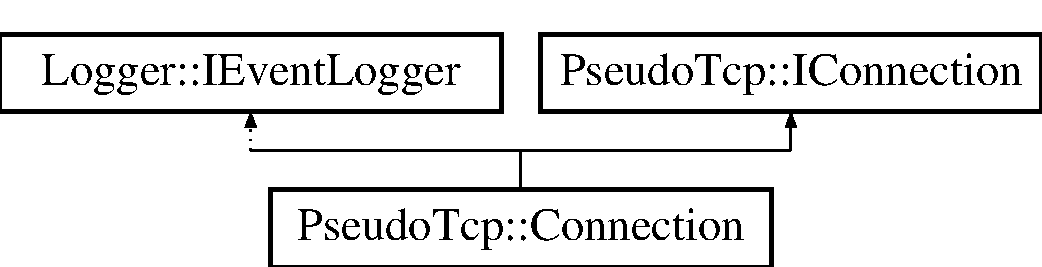
\includegraphics[height=2cm]{classPseudoTcp_1_1Connection}
\end{center}
\end{figure}
\subsection*{Public Member Functions}
\begin{DoxyCompactItemize}
\item 
\hypertarget{classPseudoTcp_1_1Connection_a73ba287568e0a03ae4957fcdce18582a}{
{\bfseries Connection} (int \hyperlink{classPseudoTcp_1_1Connection_a9baee02141ab1e3239f42c381816d70f}{id})}
\label{classPseudoTcp_1_1Connection_a73ba287568e0a03ae4957fcdce18582a}

\item 
\hypertarget{classPseudoTcp_1_1Connection_a5e97daf2c75fd93e8903403f7b187332}{
{\bfseries Connection} (int \hyperlink{classPseudoTcp_1_1Connection_a9baee02141ab1e3239f42c381816d70f}{id}, \hyperlink{classPseudoTcp_1_1IMsgHandler}{IMsgHandler} $\ast$\hyperlink{classPseudoTcp_1_1Connection_a48abbd96a00e8b85c2c6d57174956520}{msgHandler})}
\label{classPseudoTcp_1_1Connection_a5e97daf2c75fd93e8903403f7b187332}

\item 
\hypertarget{classPseudoTcp_1_1Connection_a01510ce35200ac597f6aace7a1e88efc}{
void \hyperlink{classPseudoTcp_1_1Connection_a01510ce35200ac597f6aace7a1e88efc}{SetId} (int \hyperlink{classPseudoTcp_1_1Connection_a9baee02141ab1e3239f42c381816d70f}{id})}
\label{classPseudoTcp_1_1Connection_a01510ce35200ac597f6aace7a1e88efc}

\begin{DoxyCompactList}\small\item\em Property Id is just for debugging purposes. \item\end{DoxyCompactList}\item 
\hypertarget{classPseudoTcp_1_1Connection_a309b5f8133ac8122f99ff23ff71004e1}{
virtual int \hyperlink{classPseudoTcp_1_1Connection_a309b5f8133ac8122f99ff23ff71004e1}{GetId} () const }
\label{classPseudoTcp_1_1Connection_a309b5f8133ac8122f99ff23ff71004e1}

\begin{DoxyCompactList}\small\item\em Property Id is just for debugging purposes. \item\end{DoxyCompactList}\item 
\hypertarget{classPseudoTcp_1_1Connection_aabf6e8aa15f35ba66039f23569f64626}{
void \hyperlink{classPseudoTcp_1_1Connection_aabf6e8aa15f35ba66039f23569f64626}{SetOtherHalf} (\hyperlink{classPseudoTcp_1_1Connection}{Connection} $\ast$\hyperlink{classPseudoTcp_1_1Connection_ac8324269b61373b2084ce2bd13cde979}{otherHalf})}
\label{classPseudoTcp_1_1Connection_aabf6e8aa15f35ba66039f23569f64626}

\begin{DoxyCompactList}\small\item\em Property OtherHalf points to the other \hyperlink{classPseudoTcp_1_1Connection}{Connection} object. \item\end{DoxyCompactList}\item 
\hypertarget{classPseudoTcp_1_1Connection_af0205c16aaed4f8cf890c04cb1afff79}{
\hyperlink{classPseudoTcp_1_1Connection}{Connection} $\ast$ \hyperlink{classPseudoTcp_1_1Connection_af0205c16aaed4f8cf890c04cb1afff79}{GetOtherHalf} () const }
\label{classPseudoTcp_1_1Connection_af0205c16aaed4f8cf890c04cb1afff79}

\begin{DoxyCompactList}\small\item\em Property OtherHalf points to the other \hyperlink{classPseudoTcp_1_1Connection}{Connection} object. \item\end{DoxyCompactList}\item 
\hypertarget{classPseudoTcp_1_1Connection_a8a30ac2a4127fb80437b68ead090fb07}{
void \hyperlink{classPseudoTcp_1_1Connection_a8a30ac2a4127fb80437b68ead090fb07}{SetMsgHandler} (\hyperlink{classPseudoTcp_1_1IMsgHandler}{IMsgHandler} $\ast$\hyperlink{classPseudoTcp_1_1Connection_a48abbd96a00e8b85c2c6d57174956520}{msgHandler})}
\label{classPseudoTcp_1_1Connection_a8a30ac2a4127fb80437b68ead090fb07}

\begin{DoxyCompactList}\small\item\em Property MsgHandler tells who to forward incoming messages to. \item\end{DoxyCompactList}\item 
\hypertarget{classPseudoTcp_1_1Connection_ac3557ef20de80b18c0730f9fa0ad6752}{
\hyperlink{classPseudoTcp_1_1IMsgHandler}{IMsgHandler} $\ast$ \hyperlink{classPseudoTcp_1_1Connection_ac3557ef20de80b18c0730f9fa0ad6752}{GetMsgHandler} () const }
\label{classPseudoTcp_1_1Connection_ac3557ef20de80b18c0730f9fa0ad6752}

\begin{DoxyCompactList}\small\item\em Property MsgHandler tells who to forward incoming messages to. \item\end{DoxyCompactList}\item 
\hypertarget{classPseudoTcp_1_1Connection_adfed6f5dc37e5eaf919b465886b0f11d}{
int \hyperlink{classPseudoTcp_1_1Connection_adfed6f5dc37e5eaf919b465886b0f11d}{sendMessage} (\hyperlink{classPseudoTcp_1_1Message}{Message} $\ast$msg)}
\label{classPseudoTcp_1_1Connection_adfed6f5dc37e5eaf919b465886b0f11d}

\begin{DoxyCompactList}\small\item\em Send message to other half of connection. \item\end{DoxyCompactList}\item 
\hypertarget{classPseudoTcp_1_1Connection_a56fd24c36d1715f1a19134457a0397d2}{
int \hyperlink{classPseudoTcp_1_1Connection_a56fd24c36d1715f1a19134457a0397d2}{incomingMessage} (\hyperlink{classPseudoTcp_1_1Message}{Message} msg)}
\label{classPseudoTcp_1_1Connection_a56fd24c36d1715f1a19134457a0397d2}

\begin{DoxyCompactList}\small\item\em a message arrives from other half of connection, notify MsgHandler \item\end{DoxyCompactList}\item 
\hypertarget{classPseudoTcp_1_1Connection_ace88510ecc921611cde9e56c07c65a35}{
std::string \hyperlink{classPseudoTcp_1_1Connection_ace88510ecc921611cde9e56c07c65a35}{logString} ()}
\label{classPseudoTcp_1_1Connection_ace88510ecc921611cde9e56c07c65a35}

\begin{DoxyCompactList}\small\item\em IEventLogger function. \item\end{DoxyCompactList}\item 
\hypertarget{classPseudoTcp_1_1Connection_ab1ceffdba79e19f1fc25eff2b79d05b3}{
std::string \hyperlink{classPseudoTcp_1_1Connection_ab1ceffdba79e19f1fc25eff2b79d05b3}{GetLogName} ()}
\label{classPseudoTcp_1_1Connection_ab1ceffdba79e19f1fc25eff2b79d05b3}

\begin{DoxyCompactList}\small\item\em IEventLogger function. \item\end{DoxyCompactList}\item 
virtual bool \hyperlink{classPseudoTcp_1_1Connection_aaa3f50be412caa3c5970fd5ca3d930c0}{losePacket} (\hyperlink{classPseudoTcp_1_1Message}{Message} $\ast$msg)
\begin{DoxyCompactList}\small\item\em For simulating lost packets. \item\end{DoxyCompactList}\end{DoxyCompactItemize}
\subsection*{Static Public Member Functions}
\begin{DoxyCompactItemize}
\item 
\hypertarget{classPseudoTcp_1_1Connection_a5cd5c700ba9aaca941b6f6ef198a620b}{
static void \hyperlink{classPseudoTcp_1_1Connection_a5cd5c700ba9aaca941b6f6ef198a620b}{connectConnectionPair} (\hyperlink{classPseudoTcp_1_1Connection}{Connection} $\ast$c1, \hyperlink{classPseudoTcp_1_1Connection}{Connection} $\ast$c2)}
\label{classPseudoTcp_1_1Connection_a5cd5c700ba9aaca941b6f6ef198a620b}

\begin{DoxyCompactList}\small\item\em A static function for connection two \hyperlink{classPseudoTcp_1_1Connection}{Connection} objects to each other. \item\end{DoxyCompactList}\end{DoxyCompactItemize}
\subsection*{Protected Member Functions}
\begin{DoxyCompactItemize}
\item 
\hypertarget{classPseudoTcp_1_1Connection_a61cdf90cae14c6108dc9b8382705cb79}{
void {\bfseries startSendingThread} ()}
\label{classPseudoTcp_1_1Connection_a61cdf90cae14c6108dc9b8382705cb79}

\item 
\hypertarget{classPseudoTcp_1_1Connection_af2b81f6a75b4c0dbd0306721ccf1d599}{
void {\bfseries sendMessages} ()}
\label{classPseudoTcp_1_1Connection_af2b81f6a75b4c0dbd0306721ccf1d599}

\end{DoxyCompactItemize}
\subsection*{Protected Attributes}
\begin{DoxyCompactItemize}
\item 
\hypertarget{classPseudoTcp_1_1Connection_a9baee02141ab1e3239f42c381816d70f}{
int \hyperlink{classPseudoTcp_1_1Connection_a9baee02141ab1e3239f42c381816d70f}{id}}
\label{classPseudoTcp_1_1Connection_a9baee02141ab1e3239f42c381816d70f}

\begin{DoxyCompactList}\small\item\em Property Id. \item\end{DoxyCompactList}\item 
\hypertarget{classPseudoTcp_1_1Connection_ac8324269b61373b2084ce2bd13cde979}{
\hyperlink{classPseudoTcp_1_1Connection}{Connection} $\ast$ \hyperlink{classPseudoTcp_1_1Connection_ac8324269b61373b2084ce2bd13cde979}{otherHalf}}
\label{classPseudoTcp_1_1Connection_ac8324269b61373b2084ce2bd13cde979}

\begin{DoxyCompactList}\small\item\em Property OtherHalf. \item\end{DoxyCompactList}\item 
\hypertarget{classPseudoTcp_1_1Connection_a48abbd96a00e8b85c2c6d57174956520}{
\hyperlink{classPseudoTcp_1_1IMsgHandler}{IMsgHandler} $\ast$ \hyperlink{classPseudoTcp_1_1Connection_a48abbd96a00e8b85c2c6d57174956520}{msgHandler}}
\label{classPseudoTcp_1_1Connection_a48abbd96a00e8b85c2c6d57174956520}

\begin{DoxyCompactList}\small\item\em Property MsgHandler. \item\end{DoxyCompactList}\item 
\hypertarget{classPseudoTcp_1_1Connection_a17349e4876f32fce12e2875cb2c6781a}{
int \hyperlink{classPseudoTcp_1_1Connection_a17349e4876f32fce12e2875cb2c6781a}{packetNumber}}
\label{classPseudoTcp_1_1Connection_a17349e4876f32fce12e2875cb2c6781a}

\begin{DoxyCompactList}\small\item\em Which packet number is about to be sent. \item\end{DoxyCompactList}\item 
\hypertarget{classPseudoTcp_1_1Connection_a53276de3f2fdbbf89de4cf10c85a0b4c}{
std::deque$<$ \hyperlink{classPseudoTcp_1_1Message}{Message} $>$ \hyperlink{classPseudoTcp_1_1Connection_a53276de3f2fdbbf89de4cf10c85a0b4c}{messagesToSend}}
\label{classPseudoTcp_1_1Connection_a53276de3f2fdbbf89de4cf10c85a0b4c}

\begin{DoxyCompactList}\small\item\em Shared buffer for sending thread. \item\end{DoxyCompactList}\item 
\hypertarget{classPseudoTcp_1_1Connection_aeb4d5aa737c4e972355aaa23870289e6}{
boost::shared\_\-ptr$<$ boost::thread $>$ {\bfseries sendingThread}}
\label{classPseudoTcp_1_1Connection_aeb4d5aa737c4e972355aaa23870289e6}

\item 
\hypertarget{classPseudoTcp_1_1Connection_ae4a518d298dab48493c1a37895c01342}{
boost::mutex {\bfseries messagesMutex}}
\label{classPseudoTcp_1_1Connection_ae4a518d298dab48493c1a37895c01342}

\item 
\hypertarget{classPseudoTcp_1_1Connection_aa1720cbec441514dbfe72699975d3f4b}{
volatile bool {\bfseries stopThread}}
\label{classPseudoTcp_1_1Connection_aa1720cbec441514dbfe72699975d3f4b}

\end{DoxyCompactItemize}


\subsection{Detailed Description}
A \hyperlink{classPseudoTcp_1_1Connection}{Connection} is what actually sends (or simulates sending of) a \hyperlink{classPseudoTcp_1_1Message}{Message}. A \hyperlink{classPseudoTcp_1_1Connection}{Connection} is really a half-\/connection; it has a pointer to it's other half

When 'send' is called, it forwards the message to other half. When receives incomingMessage from other half, forwards to \hyperlink{classPseudoTcp_1_1Message}{Message} handler.

Generally a \hyperlink{classPseudoTcp_1_1PseudoTcpTx}{PseudoTcpTx} object will call 'send', while a \hyperlink{classPseudoTcp_1_1PseudoTcpRx}{PseudoTcpRx} object will handle incoming messages.

The 'send' part can simulate network problems by losing, delaying, or duplicating messages.


\begin{DoxyParams}{Parameters}
\item[{\em id}]An id for the connection, can be useful in debugging. \end{DoxyParams}


\subsection{Member Function Documentation}
\hypertarget{classPseudoTcp_1_1Connection_aaa3f50be412caa3c5970fd5ca3d930c0}{
\index{PseudoTcp::Connection@{PseudoTcp::Connection}!losePacket@{losePacket}}
\index{losePacket@{losePacket}!PseudoTcp::Connection@{PseudoTcp::Connection}}
\subsubsection[{losePacket}]{\setlength{\rightskip}{0pt plus 5cm}virtual bool PseudoTcp::Connection::losePacket ({\bf Message} $\ast$ {\em msg})\hspace{0.3cm}{\ttfamily  \mbox{[}inline, virtual\mbox{]}}}}
\label{classPseudoTcp_1_1Connection_aaa3f50be412caa3c5970fd5ca3d930c0}


For simulating lost packets. 

If returns true, the message is not sent. Base class default always return false, i.e. no simulated losses. 
\begin{DoxyParams}{Parameters}
\item[{\em msg}]The \hyperlink{classPseudoTcp_1_1Message}{Message} which would be sent, for the possibility that the loss could depend on the \hyperlink{classPseudoTcp_1_1Message}{Message} number or content. \end{DoxyParams}
\begin{DoxyReturn}{Returns}

\end{DoxyReturn}


The documentation for this class was generated from the following files:\begin{DoxyCompactItemize}
\item 
Connection.hpp\item 
Connection.cpp\end{DoxyCompactItemize}

\hypertarget{classLogger_1_1Event}{
\section{Logger::Event Class Reference}
\label{classLogger_1_1Event}\index{Logger::Event@{Logger::Event}}
}
\subsection*{Public Member Functions}
\begin{DoxyCompactItemize}
\item 
\hypertarget{classLogger_1_1Event_a569b0d27277323521272decb2fc20ec8}{
{\bfseries Event} (std::string name, std::string event, std::string objectState)}
\label{classLogger_1_1Event_a569b0d27277323521272decb2fc20ec8}

\item 
\hypertarget{classLogger_1_1Event_abab783d4e89f6cab75c834644ffb9f88}{
void {\bfseries SetState} (std::string state)}
\label{classLogger_1_1Event_abab783d4e89f6cab75c834644ffb9f88}

\item 
\hypertarget{classLogger_1_1Event_aecbe9812cd4bee4891bcbe0e9b06ff5f}{
std::string {\bfseries GetState} () const }
\label{classLogger_1_1Event_aecbe9812cd4bee4891bcbe0e9b06ff5f}

\item 
\hypertarget{classLogger_1_1Event_a80070cec3b7a9e21a7d7a33df822409d}{
void {\bfseries SetEvent} (std::string event)}
\label{classLogger_1_1Event_a80070cec3b7a9e21a7d7a33df822409d}

\item 
\hypertarget{classLogger_1_1Event_a810c30f86a5ad9954404d4db9d11aa15}{
std::string {\bfseries GetEvent} () const }
\label{classLogger_1_1Event_a810c30f86a5ad9954404d4db9d11aa15}

\item 
\hypertarget{classLogger_1_1Event_ab3a3356f021232f48b236ded5bd6fe8e}{
void {\bfseries SetName} (std::string name)}
\label{classLogger_1_1Event_ab3a3356f021232f48b236ded5bd6fe8e}

\item 
\hypertarget{classLogger_1_1Event_a82bce63e60aef67c4b9cd4ffe9b597ed}{
std::string {\bfseries GetName} () const }
\label{classLogger_1_1Event_a82bce63e60aef67c4b9cd4ffe9b597ed}

\end{DoxyCompactItemize}
\subsection*{Friends}
\begin{DoxyCompactItemize}
\item 
\hypertarget{classLogger_1_1Event_aea8506a03c80dc0e72b3e3f53d8d3c74}{
std::ostream \& {\bfseries operator$<$$<$} (std::ostream \&o, \hyperlink{classLogger_1_1Event}{Event} const \&ev)}
\label{classLogger_1_1Event_aea8506a03c80dc0e72b3e3f53d8d3c74}

\end{DoxyCompactItemize}


The documentation for this class was generated from the following file:\begin{DoxyCompactItemize}
\item 
Event.hpp\end{DoxyCompactItemize}

\hypertarget{classLogger_1_1EventLogger}{
\section{Logger::EventLogger Class Reference}
\label{classLogger_1_1EventLogger}\index{Logger::EventLogger@{Logger::EventLogger}}
}


{\ttfamily \#include $<$EventLogger.hpp$>$}

\subsection*{Public Member Functions}
\begin{DoxyCompactItemize}
\item 
\hypertarget{classLogger_1_1EventLogger_af7556a247349b831fc2286388651b519}{
void {\bfseries addEvent} (\hyperlink{classLogger_1_1IEventLogger}{IEventLogger} $\ast$object, std::string event)}
\label{classLogger_1_1EventLogger_af7556a247349b831fc2286388651b519}

\item 
\hypertarget{classLogger_1_1EventLogger_a4c3d63cf1b7ee732e440e92af220de7c}{
void {\bfseries clearEvents} ()}
\label{classLogger_1_1EventLogger_a4c3d63cf1b7ee732e440e92af220de7c}

\item 
\hypertarget{classLogger_1_1EventLogger_ad34b4fde8d58e32a0804a92f70b34413}{
void {\bfseries outputEvents} (std::ostream \&stream)}
\label{classLogger_1_1EventLogger_ad34b4fde8d58e32a0804a92f70b34413}

\item 
\hypertarget{classLogger_1_1EventLogger_a9d133349096938911223839726e6f29c}{
void {\bfseries outputEvents} (std::ostream \&stream, std::string obName)}
\label{classLogger_1_1EventLogger_a9d133349096938911223839726e6f29c}

\item 
\hypertarget{classLogger_1_1EventLogger_a18fc6a9cf8737c29942bca04449e89f3}{
void {\bfseries persistEvents} (std::string path)}
\label{classLogger_1_1EventLogger_a18fc6a9cf8737c29942bca04449e89f3}

\item 
\hypertarget{classLogger_1_1EventLogger_a2b255bd3a782d86c529e7b4891388a60}{
void {\bfseries setIndentLevel} (std::string obName, int indent)}
\label{classLogger_1_1EventLogger_a2b255bd3a782d86c529e7b4891388a60}

\item 
\hypertarget{classLogger_1_1EventLogger_ac30dc3b608680a6c60f183c49c541353}{
void {\bfseries setEventLevel} (int eventLevel)}
\label{classLogger_1_1EventLogger_ac30dc3b608680a6c60f183c49c541353}

\item 
\hypertarget{classLogger_1_1EventLogger_a80a0f5bacbb74f5bff8c3cc4b77ed568}{
int {\bfseries getEventLevel} () const }
\label{classLogger_1_1EventLogger_a80a0f5bacbb74f5bff8c3cc4b77ed568}

\end{DoxyCompactItemize}
\subsection*{Static Public Member Functions}
\begin{DoxyCompactItemize}
\item 
\hypertarget{classLogger_1_1EventLogger_a9a4a948fbe302ad0cc7376725d4a1c5b}{
static \hyperlink{classLogger_1_1EventLogger}{EventLogger} $\ast$ {\bfseries glob} ()}
\label{classLogger_1_1EventLogger_a9a4a948fbe302ad0cc7376725d4a1c5b}

\item 
\hypertarget{classLogger_1_1EventLogger_a62f3ab4b10a9d804606cd62193e09716}{
static void {\bfseries setGlob} (\hyperlink{classLogger_1_1EventLogger}{EventLogger} $\ast$logger)}
\label{classLogger_1_1EventLogger_a62f3ab4b10a9d804606cd62193e09716}

\item 
\hypertarget{classLogger_1_1EventLogger_a0033da67870e179d920672a43da8b0f2}{
static void {\bfseries addEventG} (int level, \hyperlink{classLogger_1_1IEventLogger}{IEventLogger} $\ast$object, std::string event)}
\label{classLogger_1_1EventLogger_a0033da67870e179d920672a43da8b0f2}

\end{DoxyCompactItemize}


\subsection{Detailed Description}
\hyperlink{classLogger_1_1EventLogger}{EventLogger} is for debugging. Keeps track of events logged by \hyperlink{classLogger_1_1IEventLogger}{IEventLogger} objects. 

The documentation for this class was generated from the following files:\begin{DoxyCompactItemize}
\item 
EventLogger.hpp\item 
EventLogger.cpp\end{DoxyCompactItemize}

\hypertarget{classIceConnection}{
\section{IceConnection Class Reference}
\label{classIceConnection}\index{IceConnection@{IceConnection}}
}
Inheritance diagram for IceConnection:\begin{figure}[H]
\begin{center}
\leavevmode
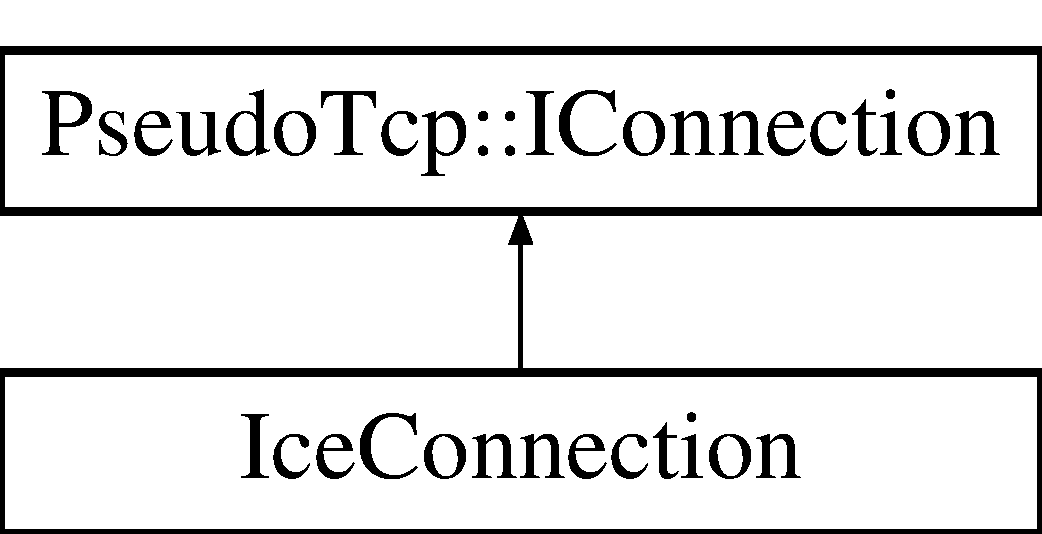
\includegraphics[height=2cm]{classIceConnection}
\end{center}
\end{figure}
\subsection*{Public Member Functions}
\begin{DoxyCompactItemize}
\item 
\hypertarget{classIceConnection_ae55802559fd5a75ad33486343a94a558}{
{\bfseries IceConnection} (\hyperlink{structP2pConnection}{P2pConnection} $\ast$conn)}
\label{classIceConnection_ae55802559fd5a75ad33486343a94a558}

\item 
\hypertarget{classIceConnection_ae2d71cdc1d53c4a7c8e55c24e31a2975}{
virtual void \hyperlink{classIceConnection_ae2d71cdc1d53c4a7c8e55c24e31a2975}{SetMsgHandler} (\hyperlink{classPseudoTcp_1_1IMsgHandler}{PseudoTcp::IMsgHandler} $\ast$msgHandler)}
\label{classIceConnection_ae2d71cdc1d53c4a7c8e55c24e31a2975}

\begin{DoxyCompactList}\small\item\em Property MsgHandler tells who to forward incoming messages to. \item\end{DoxyCompactList}\item 
\hypertarget{classIceConnection_a7da6f8856993f364ffae69058f0f0ce9}{
virtual \hyperlink{classPseudoTcp_1_1IMsgHandler}{PseudoTcp::IMsgHandler} $\ast$ \hyperlink{classIceConnection_a7da6f8856993f364ffae69058f0f0ce9}{GetMsgHandler} () const }
\label{classIceConnection_a7da6f8856993f364ffae69058f0f0ce9}

\begin{DoxyCompactList}\small\item\em Property MsgHandler tells who to forward incoming messages to. \item\end{DoxyCompactList}\item 
\hypertarget{classIceConnection_a195847a0829721e04e506bb64e5f904e}{
virtual int \hyperlink{classIceConnection_a195847a0829721e04e506bb64e5f904e}{sendMessage} (\hyperlink{classPseudoTcp_1_1Message}{PseudoTcp::Message} $\ast$msg)}
\label{classIceConnection_a195847a0829721e04e506bb64e5f904e}

\begin{DoxyCompactList}\small\item\em Send message to other half of connection. \item\end{DoxyCompactList}\item 
\hypertarget{classIceConnection_a475f6891e8aaeb44aa95f52c4961073a}{
virtual int \hyperlink{classIceConnection_a475f6891e8aaeb44aa95f52c4961073a}{incomingMessage} (\hyperlink{classPseudoTcp_1_1Message}{PseudoTcp::Message} msg)}
\label{classIceConnection_a475f6891e8aaeb44aa95f52c4961073a}

\begin{DoxyCompactList}\small\item\em a message arrives from other half of connection, notify MsgHandler \item\end{DoxyCompactList}\item 
\hypertarget{classIceConnection_a9f105aee4fe5d2079021c0e076a8f8bc}{
virtual int {\bfseries GetId} () const }
\label{classIceConnection_a9f105aee4fe5d2079021c0e076a8f8bc}

\item 
\hypertarget{classIceConnection_a7397be107c4a18c0fe288ce59e99991a}{
virtual void \hyperlink{classIceConnection_a7397be107c4a18c0fe288ce59e99991a}{registerThread} ()}
\label{classIceConnection_a7397be107c4a18c0fe288ce59e99991a}

\begin{DoxyCompactList}\small\item\em Horrible hack, made necessary by exigencies of pjnat. \item\end{DoxyCompactList}\item 
\hypertarget{classIceConnection_ab8d85a088dce0a5637db693c2d7aeb6d}{
int {\bfseries incomingRawMessage} (char $\ast$msg, int length)}
\label{classIceConnection_ab8d85a088dce0a5637db693c2d7aeb6d}

\end{DoxyCompactItemize}


The documentation for this class was generated from the following files:\begin{DoxyCompactItemize}
\item 
IceConnection.hpp\item 
IceConnection.cpp\end{DoxyCompactItemize}

\hypertarget{classIceWrapper}{
\section{IceWrapper Class Reference}
\label{classIceWrapper}\index{IceWrapper@{IceWrapper}}
}


{\ttfamily \#include $<$IceWrapper.hpp$>$}

\subsection*{Public Member Functions}
\begin{DoxyCompactItemize}
\item 
\hypertarget{classIceWrapper_a2957d299badf1008d3153cd5fd317918}{
{\bfseries IceWrapper} (const \hyperlink{classIceWrapper}{IceWrapper} \&orig)}
\label{classIceWrapper_a2957d299badf1008d3153cd5fd317918}

\item 
\hypertarget{classIceWrapper_a9d42e24532ed731e52ee59988200ad52}{
void \hyperlink{classIceWrapper_a9d42e24532ed731e52ee59988200ad52}{SetName} (std::string name)}
\label{classIceWrapper_a9d42e24532ed731e52ee59988200ad52}

\begin{DoxyCompactList}\small\item\em accessor for Name property, used for debugging \item\end{DoxyCompactList}\item 
\hypertarget{classIceWrapper_a7d2ada37e29bf229edc0fb3e05151b1d}{
std::string \hyperlink{classIceWrapper_a7d2ada37e29bf229edc0fb3e05151b1d}{GetName} () const }
\label{classIceWrapper_a7d2ada37e29bf229edc0fb3e05151b1d}

\begin{DoxyCompactList}\small\item\em accessor for Name property, used for debugging \item\end{DoxyCompactList}\item 
void \hyperlink{classIceWrapper_a9e34cb1f8e4a8b0361cb926c57971cab}{init} (const char $\ast$userName, int service, const char $\ast$rsIp, const char $\ast$rsPort)
\item 
void \hyperlink{classIceWrapper_a9577eeda39e60b4abc835c3ce81604f8}{getConn} (std::string toUser, int service)
\item 
void \hyperlink{classIceWrapper_a35ad9141a6f4a9f57f842c9f807f99bc}{send} (struct \hyperlink{structP2pConnection}{P2pConnection} $\ast$conn, std::string msg)
\item 
char $\ast$ \hyperlink{classIceWrapper_a7c19df1031dcd86d2133c5a179bb7ece}{getUsers} ()
\item 
bool \hyperlink{classIceWrapper_a648c6cda7c64d23fa210e6e62609644d}{usersChanged} ()
\item 
void \hyperlink{classIceWrapper_a1e68094e92efc427f584c682c8a470fb}{requestUsers} ()
\end{DoxyCompactItemize}
\subsection*{Static Public Member Functions}
\begin{DoxyCompactItemize}
\item 
\hypertarget{classIceWrapper_abd014f6ec26849dac26d38ba147d7240}{
static void \hyperlink{classIceWrapper_abd014f6ec26849dac26d38ba147d7240}{OnNewConnection} (struct \hyperlink{structP2pConnection}{P2pConnection} $\ast$conn)}
\label{classIceWrapper_abd014f6ec26849dac26d38ba147d7240}

\begin{DoxyCompactList}\small\item\em callback handler \item\end{DoxyCompactList}\item 
\hypertarget{classIceWrapper_abee757e1e75c9899efab4de089fbdd3a}{
static void \hyperlink{classIceWrapper_abee757e1e75c9899efab4de089fbdd3a}{OnIncomingMessage} (struct \hyperlink{structP2pConnection}{P2pConnection} $\ast$conn, char $\ast$msg, unsigned size)}
\label{classIceWrapper_abee757e1e75c9899efab4de089fbdd3a}

\begin{DoxyCompactList}\small\item\em callback handler \item\end{DoxyCompactList}\item 
\hypertarget{classIceWrapper_a5278b80ee2ca85106989f6f4c5326d2a}{
static int \hyperlink{classIceWrapper_a5278b80ee2ca85106989f6f4c5326d2a}{OnNewConnectionRequest} (struct \hyperlink{structP2pConnection}{P2pConnection} $\ast$conn)}
\label{classIceWrapper_a5278b80ee2ca85106989f6f4c5326d2a}

\begin{DoxyCompactList}\small\item\em callback handler \item\end{DoxyCompactList}\item 
\hypertarget{classIceWrapper_ad5e9159fda434266b08d5e060ce8072e}{
static void \hyperlink{classIceWrapper_ad5e9159fda434266b08d5e060ce8072e}{OnNewUsers} (char $\ast$rsUsersString)}
\label{classIceWrapper_ad5e9159fda434266b08d5e060ce8072e}

\begin{DoxyCompactList}\small\item\em callback handler \item\end{DoxyCompactList}\item 
static \hyperlink{classIceConnection}{IceConnection} $\ast$ \hyperlink{classIceWrapper_aa0cecd8091a65ccbfbe48c2397532e42}{getConnectionOfUser} (std::string userName)
\item 
static \hyperlink{classPseudoTcp_1_1MessageDispatcher}{PseudoTcp::MessageDispatcher} $\ast$ \hyperlink{classIceWrapper_a625864eb115efac6d31ea041f8093a77}{getMdOfUser} (std::string userName)
\item 
static const char $\ast$ \hyperlink{classIceWrapper_a34441a1215d0eb306b2227a9881609bd}{getInput} ()
\item 
static const char $\ast$ \hyperlink{classIceWrapper_a6e73ef401f985702be9d97abdbb1eb06}{getInput} (char $\ast$from)
\end{DoxyCompactItemize}
\subsection*{Static Public Attributes}
\begin{DoxyCompactItemize}
\item 
\hypertarget{classIceWrapper_a71005c441f47e761cb4d0e2bb68758ca}{
static bool {\bfseries Verbose} = false}
\label{classIceWrapper_a71005c441f47e761cb4d0e2bb68758ca}

\end{DoxyCompactItemize}


\subsection{Detailed Description}
The \hyperlink{classIceWrapper}{IceWrapper} class furnishes a C++ interface to the low-\/level C functionality provided by the p2pConnApi.c and rsComm.c files. \hyperlink{classIceWrapper}{IceWrapper} provides a facade to C++ for invoking the low-\/level ice functions. It uses static functions for the callbacks.

For each low-\/level connection (\hyperlink{structP2pConnection}{P2pConnection}) created, \hyperlink{classIceWrapper}{IceWrapper} creates an \hyperlink{classIceConnection}{IceConnection} and a MessageDispatcher. It keeps two maps which relate the userName to the relative \hyperlink{classIceConnection}{IceConnection} and MessageDispatcher.

\hyperlink{classIceWrapper}{IceWrapper} also supplies a function which scans all existing MessageDispatchers to see if any have input waiting. 

\subsection{Member Function Documentation}
\hypertarget{classIceWrapper_a9577eeda39e60b4abc835c3ce81604f8}{
\index{IceWrapper@{IceWrapper}!getConn@{getConn}}
\index{getConn@{getConn}!IceWrapper@{IceWrapper}}
\subsubsection[{getConn}]{\setlength{\rightskip}{0pt plus 5cm}void IceWrapper::getConn (std::string {\em toUser}, \/  int {\em service})}}
\label{classIceWrapper_a9577eeda39e60b4abc835c3ce81604f8}
Request a connection to a user for an application 
\begin{DoxyParams}{Parameters}
\item[{\em toUser}]user to connect to \item[{\em service}]MyMed application number \end{DoxyParams}
\hypertarget{classIceWrapper_aa0cecd8091a65ccbfbe48c2397532e42}{
\index{IceWrapper@{IceWrapper}!getConnectionOfUser@{getConnectionOfUser}}
\index{getConnectionOfUser@{getConnectionOfUser}!IceWrapper@{IceWrapper}}
\subsubsection[{getConnectionOfUser}]{\setlength{\rightskip}{0pt plus 5cm}{\bf IceConnection} $\ast$ IceWrapper::getConnectionOfUser (std::string {\em userName})\hspace{0.3cm}{\ttfamily  \mbox{[}static\mbox{]}}}}
\label{classIceWrapper_aa0cecd8091a65ccbfbe48c2397532e42}
Return \hyperlink{classIceConnection}{IceConnection} corresponding to user 
\begin{DoxyParams}{Parameters}
\item[{\em userName}]name of user to get connection of \end{DoxyParams}
\begin{DoxyReturn}{Returns}

\end{DoxyReturn}
\hypertarget{classIceWrapper_a6e73ef401f985702be9d97abdbb1eb06}{
\index{IceWrapper@{IceWrapper}!getInput@{getInput}}
\index{getInput@{getInput}!IceWrapper@{IceWrapper}}
\subsubsection[{getInput}]{\setlength{\rightskip}{0pt plus 5cm}const char $\ast$ IceWrapper::getInput (char $\ast$ {\em from})\hspace{0.3cm}{\ttfamily  \mbox{[}static\mbox{]}}}}
\label{classIceWrapper_a6e73ef401f985702be9d97abdbb1eb06}
Scan all MessageDispatchers, if any have input return the input. 
\begin{DoxyParams}{Parameters}
\item[{\em from}]'out' parameter will be set to userName of user who sent the input. \end{DoxyParams}
\begin{DoxyReturn}{Returns}

\end{DoxyReturn}
\hypertarget{classIceWrapper_a34441a1215d0eb306b2227a9881609bd}{
\index{IceWrapper@{IceWrapper}!getInput@{getInput}}
\index{getInput@{getInput}!IceWrapper@{IceWrapper}}
\subsubsection[{getInput}]{\setlength{\rightskip}{0pt plus 5cm}const char $\ast$ IceWrapper::getInput ()\hspace{0.3cm}{\ttfamily  \mbox{[}static\mbox{]}}}}
\label{classIceWrapper_a34441a1215d0eb306b2227a9881609bd}
Obsolete, remove \begin{DoxyReturn}{Returns}

\end{DoxyReturn}
\hypertarget{classIceWrapper_a625864eb115efac6d31ea041f8093a77}{
\index{IceWrapper@{IceWrapper}!getMdOfUser@{getMdOfUser}}
\index{getMdOfUser@{getMdOfUser}!IceWrapper@{IceWrapper}}
\subsubsection[{getMdOfUser}]{\setlength{\rightskip}{0pt plus 5cm}{\bf PseudoTcp::MessageDispatcher} $\ast$ IceWrapper::getMdOfUser (std::string {\em userName})\hspace{0.3cm}{\ttfamily  \mbox{[}static\mbox{]}}}}
\label{classIceWrapper_a625864eb115efac6d31ea041f8093a77}
Return MessageDispatcher corresponding to user 
\begin{DoxyParams}{Parameters}
\item[{\em userName}]name of user to get MessageDispatcher of \end{DoxyParams}
\begin{DoxyReturn}{Returns}

\end{DoxyReturn}
\hypertarget{classIceWrapper_a7c19df1031dcd86d2133c5a179bb7ece}{
\index{IceWrapper@{IceWrapper}!getUsers@{getUsers}}
\index{getUsers@{getUsers}!IceWrapper@{IceWrapper}}
\subsubsection[{getUsers}]{\setlength{\rightskip}{0pt plus 5cm}char $\ast$ IceWrapper::getUsers ()}}
\label{classIceWrapper_a7c19df1031dcd86d2133c5a179bb7ece}
Return the userstring received from the RS \begin{DoxyReturn}{Returns}

\end{DoxyReturn}
\hypertarget{classIceWrapper_a9e34cb1f8e4a8b0361cb926c57971cab}{
\index{IceWrapper@{IceWrapper}!init@{init}}
\index{init@{init}!IceWrapper@{IceWrapper}}
\subsubsection[{init}]{\setlength{\rightskip}{0pt plus 5cm}void IceWrapper::init (const char $\ast$ {\em userName}, \/  int {\em service}, \/  const char $\ast$ {\em rsIp}, \/  const char $\ast$ {\em rsPort})}}
\label{classIceWrapper_a9e34cb1f8e4a8b0361cb926c57971cab}
Initialization parameters for low level 
\begin{DoxyParams}{Parameters}
\item[{\em userName}]Name of user who is registering \item[{\em service}]MyMed Application number \item[{\em rsIp}]IP address of Rendezvous server \item[{\em rsPort}]Port of Rendezvous server \end{DoxyParams}
\hypertarget{classIceWrapper_a1e68094e92efc427f584c682c8a470fb}{
\index{IceWrapper@{IceWrapper}!requestUsers@{requestUsers}}
\index{requestUsers@{requestUsers}!IceWrapper@{IceWrapper}}
\subsubsection[{requestUsers}]{\setlength{\rightskip}{0pt plus 5cm}void IceWrapper::requestUsers ()}}
\label{classIceWrapper_a1e68094e92efc427f584c682c8a470fb}
Send a request to the RS for currently registered users. \hypertarget{classIceWrapper_a35ad9141a6f4a9f57f842c9f807f99bc}{
\index{IceWrapper@{IceWrapper}!send@{send}}
\index{send@{send}!IceWrapper@{IceWrapper}}
\subsubsection[{send}]{\setlength{\rightskip}{0pt plus 5cm}void IceWrapper::send (struct {\bf P2pConnection} $\ast$ {\em conn}, \/  std::string {\em msg})}}
\label{classIceWrapper_a35ad9141a6f4a9f57f842c9f807f99bc}
Send a string using a connection 
\begin{DoxyParams}{Parameters}
\item[{\em conn}]Lower level connection to use \item[{\em msg}]Message to send \end{DoxyParams}
\hypertarget{classIceWrapper_a648c6cda7c64d23fa210e6e62609644d}{
\index{IceWrapper@{IceWrapper}!usersChanged@{usersChanged}}
\index{usersChanged@{usersChanged}!IceWrapper@{IceWrapper}}
\subsubsection[{usersChanged}]{\setlength{\rightskip}{0pt plus 5cm}bool IceWrapper::usersChanged ()}}
\label{classIceWrapper_a648c6cda7c64d23fa210e6e62609644d}
Return true if userstring has been updated \begin{DoxyReturn}{Returns}

\end{DoxyReturn}


The documentation for this class was generated from the following files:\begin{DoxyCompactItemize}
\item 
IceWrapper.hpp\item 
IceWrapper.cpp\end{DoxyCompactItemize}

\hypertarget{classPseudoTcp_1_1IConnection}{
\section{PseudoTcp::IConnection Class Reference}
\label{classPseudoTcp_1_1IConnection}\index{PseudoTcp::IConnection@{PseudoTcp::IConnection}}
}
Inheritance diagram for PseudoTcp::IConnection:\begin{figure}[H]
\begin{center}
\leavevmode
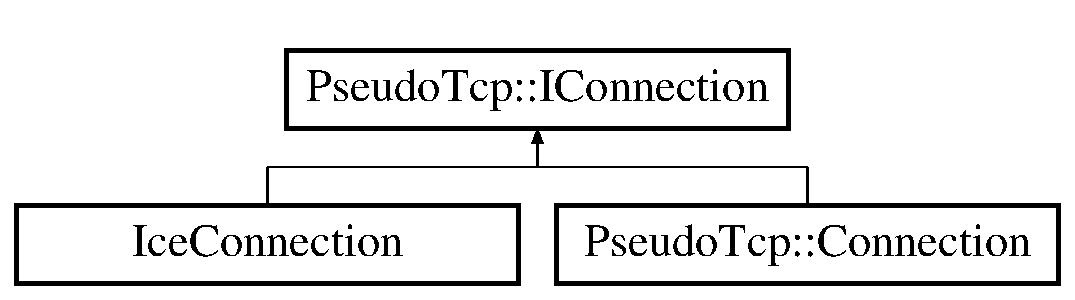
\includegraphics[height=2cm]{classPseudoTcp_1_1IConnection}
\end{center}
\end{figure}
\subsection*{Public Member Functions}
\begin{DoxyCompactItemize}
\item 
\hypertarget{classPseudoTcp_1_1IConnection_ae3b2a63ff3d75130a9ea4e9197ff6eb2}{
virtual void \hyperlink{classPseudoTcp_1_1IConnection_ae3b2a63ff3d75130a9ea4e9197ff6eb2}{SetMsgHandler} (\hyperlink{classPseudoTcp_1_1IMsgHandler}{IMsgHandler} $\ast$msgHandler)=0}
\label{classPseudoTcp_1_1IConnection_ae3b2a63ff3d75130a9ea4e9197ff6eb2}

\begin{DoxyCompactList}\small\item\em Property MsgHandler tells who to forward incoming messages to. \item\end{DoxyCompactList}\item 
\hypertarget{classPseudoTcp_1_1IConnection_adcb33b73838a97b7abcc1b8fc4ed56a2}{
virtual \hyperlink{classPseudoTcp_1_1IMsgHandler}{IMsgHandler} $\ast$ \hyperlink{classPseudoTcp_1_1IConnection_adcb33b73838a97b7abcc1b8fc4ed56a2}{GetMsgHandler} () const =0}
\label{classPseudoTcp_1_1IConnection_adcb33b73838a97b7abcc1b8fc4ed56a2}

\begin{DoxyCompactList}\small\item\em Property MsgHandler tells who to forward incoming messages to. \item\end{DoxyCompactList}\item 
\hypertarget{classPseudoTcp_1_1IConnection_a82f7a2ca2784a9c3da5bdd022aec0f59}{
virtual int \hyperlink{classPseudoTcp_1_1IConnection_a82f7a2ca2784a9c3da5bdd022aec0f59}{sendMessage} (\hyperlink{classPseudoTcp_1_1Message}{Message} $\ast$msg)=0}
\label{classPseudoTcp_1_1IConnection_a82f7a2ca2784a9c3da5bdd022aec0f59}

\begin{DoxyCompactList}\small\item\em Send message to other half of connection. \item\end{DoxyCompactList}\item 
\hypertarget{classPseudoTcp_1_1IConnection_afe96a0f5f39c83ec5b9367734529ec68}{
virtual int \hyperlink{classPseudoTcp_1_1IConnection_afe96a0f5f39c83ec5b9367734529ec68}{incomingMessage} (\hyperlink{classPseudoTcp_1_1Message}{Message} msg)=0}
\label{classPseudoTcp_1_1IConnection_afe96a0f5f39c83ec5b9367734529ec68}

\begin{DoxyCompactList}\small\item\em a message arrives from other half of connection, notify MsgHandler \item\end{DoxyCompactList}\item 
\hypertarget{classPseudoTcp_1_1IConnection_adb019cbaaa9ac27a98764a7085a67e3f}{
virtual int {\bfseries GetId} () const =0}
\label{classPseudoTcp_1_1IConnection_adb019cbaaa9ac27a98764a7085a67e3f}

\item 
\hypertarget{classPseudoTcp_1_1IConnection_a5166f14753cd7cc5ca8e20e701812f0c}{
virtual void \hyperlink{classPseudoTcp_1_1IConnection_a5166f14753cd7cc5ca8e20e701812f0c}{registerThread} ()=0}
\label{classPseudoTcp_1_1IConnection_a5166f14753cd7cc5ca8e20e701812f0c}

\begin{DoxyCompactList}\small\item\em Horrible hack, made necessary by exigencies of pjnat. \item\end{DoxyCompactList}\end{DoxyCompactItemize}


The documentation for this class was generated from the following file:\begin{DoxyCompactItemize}
\item 
IConnection.hpp\end{DoxyCompactItemize}

\hypertarget{classLogger_1_1IEventLogger}{
\section{Logger::IEventLogger Class Reference}
\label{classLogger_1_1IEventLogger}\index{Logger::IEventLogger@{Logger::IEventLogger}}
}
Inheritance diagram for Logger::IEventLogger:\begin{figure}[H]
\begin{center}
\leavevmode
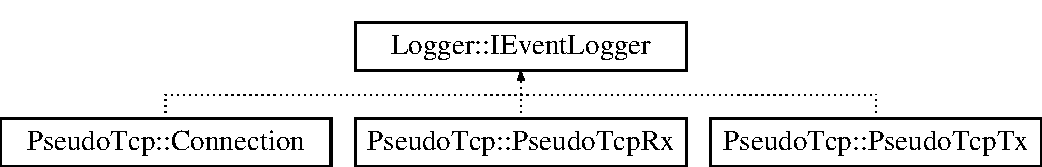
\includegraphics[height=2cm]{classLogger_1_1IEventLogger}
\end{center}
\end{figure}
\subsection*{Public Member Functions}
\begin{DoxyCompactItemize}
\item 
\hypertarget{classLogger_1_1IEventLogger_abc4749625087fc9ebcfa992cc1ee078a}{
virtual std::string {\bfseries GetLogName} ()=0}
\label{classLogger_1_1IEventLogger_abc4749625087fc9ebcfa992cc1ee078a}

\item 
\hypertarget{classLogger_1_1IEventLogger_a4ea2d0512baf7042a98bbe76a7836bd6}{
virtual std::string {\bfseries logString} ()=0}
\label{classLogger_1_1IEventLogger_a4ea2d0512baf7042a98bbe76a7836bd6}

\end{DoxyCompactItemize}


The documentation for this class was generated from the following file:\begin{DoxyCompactItemize}
\item 
IEventLogger.hpp\end{DoxyCompactItemize}

\hypertarget{classPseudoTcp_1_1IMsgHandler}{
\section{PseudoTcp::IMsgHandler Class Reference}
\label{classPseudoTcp_1_1IMsgHandler}\index{PseudoTcp::IMsgHandler@{PseudoTcp::IMsgHandler}}
}


Interface for callback from \hyperlink{classPseudoTcp_1_1Connection}{Connection} with \hyperlink{classPseudoTcp_1_1Message}{Message}.  




{\ttfamily \#include $<$IMsgHandler.hpp$>$}

Inheritance diagram for PseudoTcp::IMsgHandler:\begin{figure}[H]
\begin{center}
\leavevmode
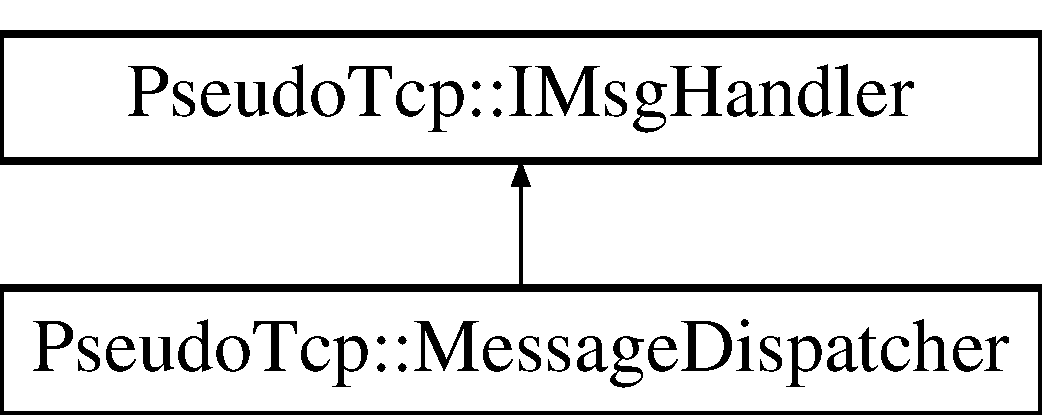
\includegraphics[height=2cm]{classPseudoTcp_1_1IMsgHandler}
\end{center}
\end{figure}
\subsection*{Public Member Functions}
\begin{DoxyCompactItemize}
\item 
\hypertarget{classPseudoTcp_1_1IMsgHandler_a489ae29ae542515d53a21eaac9af03c0}{
virtual void {\bfseries IncomingMessage} (\hyperlink{classPseudoTcp_1_1Message}{Message} $\ast$msg)=0}
\label{classPseudoTcp_1_1IMsgHandler_a489ae29ae542515d53a21eaac9af03c0}

\end{DoxyCompactItemize}


\subsection{Detailed Description}
Interface for callback from \hyperlink{classPseudoTcp_1_1Connection}{Connection} with \hyperlink{classPseudoTcp_1_1Message}{Message}. The \hyperlink{classPseudoTcp_1_1IMsgHandler}{IMsgHandler} interface serves implement a callback from the lower level \hyperlink{classPseudoTcp_1_1Connection}{Connection} to the higher level \hyperlink{classPseudoTcp_1_1MessageDispatcher}{MessageDispatcher} avoiding circular dependencies. 
\begin{DoxyParams}{Parameters}
\item[{\em msg}]The \hyperlink{classPseudoTcp_1_1Message}{Message} to handle. \end{DoxyParams}


The documentation for this class was generated from the following file:\begin{DoxyCompactItemize}
\item 
IMsgHandler.hpp\end{DoxyCompactItemize}

\hypertarget{classmymed_1_1JavaIceWrapper}{
\section{mymed::JavaIceWrapper Class Reference}
\label{classmymed_1_1JavaIceWrapper}\index{mymed::JavaIceWrapper@{mymed::JavaIceWrapper}}
}
\subsection*{Public Member Functions}
\begin{DoxyCompactItemize}
\item 
native void \hyperlink{classmymed_1_1JavaIceWrapper_acbc9014ee604c6dfbec6e1f3c1f4500e}{getConnection} (String name, int service)
\item 
native void \hyperlink{classmymed_1_1JavaIceWrapper_ae3d2b5589121f5d5f0184aea567fd4e5}{send} (String name, String msg)
\item 
native String \hyperlink{classmymed_1_1JavaIceWrapper_af9bc0222407efaa31cb5237dbc3056c2}{getUsersString} ()
\item 
native String \hyperlink{classmymed_1_1JavaIceWrapper_a800d9af066725c394979d86aabb10ba8}{getInput} ()
\item 
native String \hyperlink{classmymed_1_1JavaIceWrapper_a8a950610ddf0c69e287f6d1702b97387}{getInput} (StringBuffer from)
\item 
native int \hyperlink{classmymed_1_1JavaIceWrapper_af06e8244e449b1b5e65948ea70581d6a}{hasConnection} (String name, int service)
\end{DoxyCompactItemize}


\subsection{Detailed Description}
This class loads the library which provided peer-\/to-\/peer connections for MyMed, and furnishes a java intervace via JNI to this functionality. \begin{DoxyAuthor}{Author}
Peter Neuss 
\end{DoxyAuthor}


\subsection{Member Function Documentation}
\hypertarget{classmymed_1_1JavaIceWrapper_acbc9014ee604c6dfbec6e1f3c1f4500e}{
\index{mymed::JavaIceWrapper@{mymed::JavaIceWrapper}!getConnection@{getConnection}}
\index{getConnection@{getConnection}!mymed::JavaIceWrapper@{mymed::JavaIceWrapper}}
\subsubsection[{getConnection}]{\setlength{\rightskip}{0pt plus 5cm}native void mymed::JavaIceWrapper::getConnection (String {\em name}, \/  int {\em service})}}
\label{classmymed_1_1JavaIceWrapper_acbc9014ee604c6dfbec6e1f3c1f4500e}
Establish connection with user for an application 
\begin{DoxyParams}{Parameters}
\item[{\em name}]user to connect to \item[{\em service}]MyMed application number to use \end{DoxyParams}
\hypertarget{classmymed_1_1JavaIceWrapper_a8a950610ddf0c69e287f6d1702b97387}{
\index{mymed::JavaIceWrapper@{mymed::JavaIceWrapper}!getInput@{getInput}}
\index{getInput@{getInput}!mymed::JavaIceWrapper@{mymed::JavaIceWrapper}}
\subsubsection[{getInput}]{\setlength{\rightskip}{0pt plus 5cm}native String mymed::JavaIceWrapper::getInput (StringBuffer {\em from})}}
\label{classmymed_1_1JavaIceWrapper_a8a950610ddf0c69e287f6d1702b97387}
Scan all MessageDispatchers, if any have input return the input. 
\begin{DoxyParams}{Parameters}
\item[{\em from}]'out' parameter will be set to userName of user who sent the input. \end{DoxyParams}
\begin{DoxyReturn}{Returns}
the input 
\end{DoxyReturn}
\hypertarget{classmymed_1_1JavaIceWrapper_a800d9af066725c394979d86aabb10ba8}{
\index{mymed::JavaIceWrapper@{mymed::JavaIceWrapper}!getInput@{getInput}}
\index{getInput@{getInput}!mymed::JavaIceWrapper@{mymed::JavaIceWrapper}}
\subsubsection[{getInput}]{\setlength{\rightskip}{0pt plus 5cm}native String mymed::JavaIceWrapper::getInput ()}}
\label{classmymed_1_1JavaIceWrapper_a800d9af066725c394979d86aabb10ba8}
obsolete, do not use. \begin{DoxyReturn}{Returns}

\end{DoxyReturn}
\hypertarget{classmymed_1_1JavaIceWrapper_af9bc0222407efaa31cb5237dbc3056c2}{
\index{mymed::JavaIceWrapper@{mymed::JavaIceWrapper}!getUsersString@{getUsersString}}
\index{getUsersString@{getUsersString}!mymed::JavaIceWrapper@{mymed::JavaIceWrapper}}
\subsubsection[{getUsersString}]{\setlength{\rightskip}{0pt plus 5cm}native String mymed::JavaIceWrapper::getUsersString ()}}
\label{classmymed_1_1JavaIceWrapper_af9bc0222407efaa31cb5237dbc3056c2}
Return the userstring received from Rendezvous server \begin{DoxyReturn}{Returns}

\end{DoxyReturn}
\hypertarget{classmymed_1_1JavaIceWrapper_af06e8244e449b1b5e65948ea70581d6a}{
\index{mymed::JavaIceWrapper@{mymed::JavaIceWrapper}!hasConnection@{hasConnection}}
\index{hasConnection@{hasConnection}!mymed::JavaIceWrapper@{mymed::JavaIceWrapper}}
\subsubsection[{hasConnection}]{\setlength{\rightskip}{0pt plus 5cm}native int mymed::JavaIceWrapper::hasConnection (String {\em name}, \/  int {\em service})}}
\label{classmymed_1_1JavaIceWrapper_af06e8244e449b1b5e65948ea70581d6a}
See if there has already been a connection established to user 
\begin{DoxyParams}{Parameters}
\item[{\em name}]other user \item[{\em service}]MyMed application number \end{DoxyParams}
\begin{DoxyReturn}{Returns}
1 if there is a connection, 0 otherwise 
\end{DoxyReturn}
\hypertarget{classmymed_1_1JavaIceWrapper_ae3d2b5589121f5d5f0184aea567fd4e5}{
\index{mymed::JavaIceWrapper@{mymed::JavaIceWrapper}!send@{send}}
\index{send@{send}!mymed::JavaIceWrapper@{mymed::JavaIceWrapper}}
\subsubsection[{send}]{\setlength{\rightskip}{0pt plus 5cm}native void mymed::JavaIceWrapper::send (String {\em name}, \/  String {\em msg})}}
\label{classmymed_1_1JavaIceWrapper_ae3d2b5589121f5d5f0184aea567fd4e5}
Send a message to a user 
\begin{DoxyParams}{Parameters}
\item[{\em name}]destination user \item[{\em msg}]message to send \end{DoxyParams}


The documentation for this class was generated from the following file:\begin{DoxyCompactItemize}
\item 
mymed/JavaIceWrapper.java\end{DoxyCompactItemize}

\hypertarget{classPseudoTcp_1_1Message}{
\section{PseudoTcp::Message Class Reference}
\label{classPseudoTcp_1_1Message}\index{PseudoTcp::Message@{PseudoTcp::Message}}
}


Encapsulates the protocol format.  




{\ttfamily \#include $<$Message.hpp$>$}

\subsection*{Public Member Functions}
\begin{DoxyCompactItemize}
\item 
\hypertarget{classPseudoTcp_1_1Message_a638940a04839b0562f290f889241d024}{
{\bfseries Message} (std::vector$<$ unsigned char $>$ payload)}
\label{classPseudoTcp_1_1Message_a638940a04839b0562f290f889241d024}

\item 
\hyperlink{classPseudoTcp_1_1Message_a9adbafc6e615e070f8e0ef861a507421}{Message} (int n)
\item 
\hypertarget{classPseudoTcp_1_1Message_af505c01b16ce8a4df996328ec57e23de}{
std::vector$<$ unsigned char $>$ \& \hyperlink{classPseudoTcp_1_1Message_af505c01b16ce8a4df996328ec57e23de}{GetByteArray} ()}
\label{classPseudoTcp_1_1Message_af505c01b16ce8a4df996328ec57e23de}

\begin{DoxyCompactList}\small\item\em Returns the payload. \item\end{DoxyCompactList}\item 
\hypertarget{group__group1_gaefd21c9f3d668b1e918bed1784afab84}{
void \hyperlink{group__group1_gaefd21c9f3d668b1e918bed1784afab84}{SetAck} (bool ack)}
\label{group__group1_gaefd21c9f3d668b1e918bed1784afab84}

\begin{DoxyCompactList}\small\item\em Set whether this \hyperlink{classPseudoTcp_1_1Message}{Message} contains an Ack. \item\end{DoxyCompactList}\item 
\hypertarget{group__group1_ga6b3b9a3bccbaa08efa0ebfdbf6222581}{
bool \hyperlink{group__group1_ga6b3b9a3bccbaa08efa0ebfdbf6222581}{IsAck} () const }
\label{group__group1_ga6b3b9a3bccbaa08efa0ebfdbf6222581}

\begin{DoxyCompactList}\small\item\em true if the \hyperlink{classPseudoTcp_1_1Message}{Message} is an Ack \item\end{DoxyCompactList}\item 
\hypertarget{group__group1_gafdf542899b221aee3bbce73738d9b809}{
void \hyperlink{group__group1_gafdf542899b221aee3bbce73738d9b809}{SetNumber} (int number)}
\label{group__group1_gafdf542899b221aee3bbce73738d9b809}

\begin{DoxyCompactList}\small\item\em Number property is sequential numbering of Messages sent by a \hyperlink{classPseudoTcp_1_1PseudoTcpTx}{PseudoTcpTx}. \item\end{DoxyCompactList}\item 
\hypertarget{group__group1_gada70d38e0b9059de0d8f61fbda4adf30}{
int \hyperlink{group__group1_gada70d38e0b9059de0d8f61fbda4adf30}{GetNumber} () const }
\label{group__group1_gada70d38e0b9059de0d8f61fbda4adf30}

\begin{DoxyCompactList}\small\item\em Number property is sequential numbering of Messages sent by a \hyperlink{classPseudoTcp_1_1PseudoTcpTx}{PseudoTcpTx}. \item\end{DoxyCompactList}\item 
\hypertarget{group__group1_ga4fee4812147aa855109d0aed46a6030c}{
void \hyperlink{group__group1_ga4fee4812147aa855109d0aed46a6030c}{SetReqAck} (bool reqAck)}
\label{group__group1_ga4fee4812147aa855109d0aed46a6030c}

\begin{DoxyCompactList}\small\item\em ReqAck property determines whether this \hyperlink{classPseudoTcp_1_1Message}{Message} requests an ack. \item\end{DoxyCompactList}\item 
\hypertarget{group__group1_gae74d45f2834806fda6d72c44f651793c}{
bool \hyperlink{group__group1_gae74d45f2834806fda6d72c44f651793c}{IsReqAck} () const }
\label{group__group1_gae74d45f2834806fda6d72c44f651793c}

\begin{DoxyCompactList}\small\item\em ReqAck property determines whether this \hyperlink{classPseudoTcp_1_1Message}{Message} requests an ack. \item\end{DoxyCompactList}\item 
\hypertarget{group__group1_ga2c8aa429145e2bf950d0e1b4f25e5f1c}{
void \hyperlink{group__group1_ga2c8aa429145e2bf950d0e1b4f25e5f1c}{SetAckNumber} (int ackNumber)}
\label{group__group1_ga2c8aa429145e2bf950d0e1b4f25e5f1c}

\begin{DoxyCompactList}\small\item\em AckNumber property is the \hyperlink{classPseudoTcp_1_1Message}{Message} number of the message we are acking. \item\end{DoxyCompactList}\item 
\hypertarget{group__group1_ga5cb28e660d6cbed4a7bffbe6c2597cb9}{
int \hyperlink{group__group1_ga5cb28e660d6cbed4a7bffbe6c2597cb9}{GetAckNumber} () const }
\label{group__group1_ga5cb28e660d6cbed4a7bffbe6c2597cb9}

\begin{DoxyCompactList}\small\item\em AckNumber property is the \hyperlink{classPseudoTcp_1_1Message}{Message} number of the message we are acking. \item\end{DoxyCompactList}\item 
\hypertarget{group__group1_ga21fdfd49d1112874b860a10094f7dbe4}{
void \hyperlink{group__group1_ga21fdfd49d1112874b860a10094f7dbe4}{SetAckBase} (int ackBase)}
\label{group__group1_ga21fdfd49d1112874b860a10094f7dbe4}

\begin{DoxyCompactList}\small\item\em AckBase property represents the lowest missing \hyperlink{classPseudoTcp_1_1Message}{Message} number. \item\end{DoxyCompactList}\item 
\hypertarget{group__group1_ga18f1c004034b89226d9c29a16425e18f}{
int \hyperlink{group__group1_ga18f1c004034b89226d9c29a16425e18f}{GetAckBase} () const }
\label{group__group1_ga18f1c004034b89226d9c29a16425e18f}

\begin{DoxyCompactList}\small\item\em AckBase property represents the lowest missing \hyperlink{classPseudoTcp_1_1Message}{Message} number. \item\end{DoxyCompactList}\item 
void \hyperlink{group__group1_ga8d775b77bb73f7db77e0f8fec82b9a26}{SetLastSent} (double lastSent)
\begin{DoxyCompactList}\small\item\em LastSent property is the time of the most recent attempted send of the \hyperlink{classPseudoTcp_1_1Message}{Message}. \item\end{DoxyCompactList}\item 
\hypertarget{group__group1_ga342f652745ccf8d643991905c3c4ac0a}{
double \hyperlink{group__group1_ga342f652745ccf8d643991905c3c4ac0a}{GetLastSent} () const }
\label{group__group1_ga342f652745ccf8d643991905c3c4ac0a}

\begin{DoxyCompactList}\small\item\em LastSent property is the time of the most recent attempted send of the \hyperlink{classPseudoTcp_1_1Message}{Message}. \item\end{DoxyCompactList}\item 
std::bitset$<$ MSG\_\-WIN $>$ \hyperlink{group__group1_gaa74cf86697d336a90508f375067e02ef}{GetMsgsReceived} ()
\begin{DoxyCompactList}\small\item\em for debugging only. \item\end{DoxyCompactList}\item 
\hypertarget{group__group1_gaaf86c7594534b605b19a0f7843c02e93}{
void \hyperlink{group__group1_gaaf86c7594534b605b19a0f7843c02e93}{SetMsgsReceived} (std::bitset$<$ MSG\_\-WIN $>$ msgsReceived)}
\label{group__group1_gaaf86c7594534b605b19a0f7843c02e93}

\begin{DoxyCompactList}\small\item\em each bit represents a \hyperlink{classPseudoTcp_1_1Message}{Message} in the window, 1 if received, 0 if not \item\end{DoxyCompactList}\item 
\hypertarget{classPseudoTcp_1_1Message_a594bb615fbd8a2b617ee0123b8b0f731}{
bool \hyperlink{classPseudoTcp_1_1Message_a594bb615fbd8a2b617ee0123b8b0f731}{hasPayload} ()}
\label{classPseudoTcp_1_1Message_a594bb615fbd8a2b617ee0123b8b0f731}

\begin{DoxyCompactList}\small\item\em true if message has payload (is not just an ack) \item\end{DoxyCompactList}\item 
\hypertarget{classPseudoTcp_1_1Message_ac73b3655ae61e6140019d819383c594e}{
std::string \hyperlink{classPseudoTcp_1_1Message_ac73b3655ae61e6140019d819383c594e}{toString} () const }
\label{classPseudoTcp_1_1Message_ac73b3655ae61e6140019d819383c594e}

\begin{DoxyCompactList}\small\item\em A more detailed output then $<$$<$. \item\end{DoxyCompactList}\end{DoxyCompactItemize}
\subsection*{Static Public Attributes}
\begin{DoxyCompactItemize}
\item 
\hypertarget{classPseudoTcp_1_1Message_af700d12cf3f42af92dd2bf65cf9a20a3}{
static const int \hyperlink{classPseudoTcp_1_1Message_af700d12cf3f42af92dd2bf65cf9a20a3}{UNNUMBERED} = -\/1}
\label{classPseudoTcp_1_1Message_af700d12cf3f42af92dd2bf65cf9a20a3}

\begin{DoxyCompactList}\small\item\em Special value of property Number to indicate unitialized. \item\end{DoxyCompactList}\item 
\hypertarget{classPseudoTcp_1_1Message_a28f26b18c79f0081d076b4ff521cea37}{
static const double \hyperlink{classPseudoTcp_1_1Message_a28f26b18c79f0081d076b4ff521cea37}{NEVER\_\-SENT} = -\/1.0}
\label{classPseudoTcp_1_1Message_a28f26b18c79f0081d076b4ff521cea37}

\begin{DoxyCompactList}\small\item\em Special value of property LastSent to indicate \hyperlink{classPseudoTcp_1_1Message}{Message} has never been sent. \item\end{DoxyCompactList}\end{DoxyCompactItemize}
\subsection*{Friends}
\begin{DoxyCompactItemize}
\item 
\hypertarget{classPseudoTcp_1_1Message_ac98d07dd8f7b70e16ccb9a01abf56b9c}{
class \hyperlink{classPseudoTcp_1_1Message_ac98d07dd8f7b70e16ccb9a01abf56b9c}{boost::serialization::access}}
\label{classPseudoTcp_1_1Message_ac98d07dd8f7b70e16ccb9a01abf56b9c}

\begin{DoxyCompactList}\small\item\em Boost serialization. \item\end{DoxyCompactList}\item 
\hypertarget{classPseudoTcp_1_1Message_ab393938982c2c1738d4a96618c53e340}{
std::ostream \& {\bfseries operator$<$$<$} (std::ostream \&o, \hyperlink{classPseudoTcp_1_1Message}{Message} const \&msg)}
\label{classPseudoTcp_1_1Message_ab393938982c2c1738d4a96618c53e340}

\end{DoxyCompactItemize}


\subsection{Detailed Description}
Encapsulates the protocol format. GetByteArray returns the payload, the rest is the header. 

\subsection{Constructor \& Destructor Documentation}
\hypertarget{classPseudoTcp_1_1Message_a9adbafc6e615e070f8e0ef861a507421}{
\index{PseudoTcp::Message@{PseudoTcp::Message}!Message@{Message}}
\index{Message@{Message}!PseudoTcp::Message@{PseudoTcp::Message}}
\subsubsection[{Message}]{\setlength{\rightskip}{0pt plus 5cm}PseudoTcp::Message::Message (int {\em n})}}
\label{classPseudoTcp_1_1Message_a9adbafc6e615e070f8e0ef861a507421}
For testing purposes, create a message of length n whose elements are 'a' 
\begin{DoxyParams}{Parameters}
\item[{\em n}]\end{DoxyParams}


The documentation for this class was generated from the following files:\begin{DoxyCompactItemize}
\item 
Message.hpp\item 
Message.cpp\end{DoxyCompactItemize}

\hypertarget{classPseudoTcp_1_1MessageDispatcher}{
\section{PseudoTcp::MessageDispatcher Class Reference}
\label{classPseudoTcp_1_1MessageDispatcher}\index{PseudoTcp::MessageDispatcher@{PseudoTcp::MessageDispatcher}}
}


Top level \hyperlink{namespacePseudoTcp}{PseudoTcp} object, which contains TX and TX parts.  




{\ttfamily \#include $<$MessageDispatcher.hpp$>$}

Inheritance diagram for PseudoTcp::MessageDispatcher:\begin{figure}[H]
\begin{center}
\leavevmode
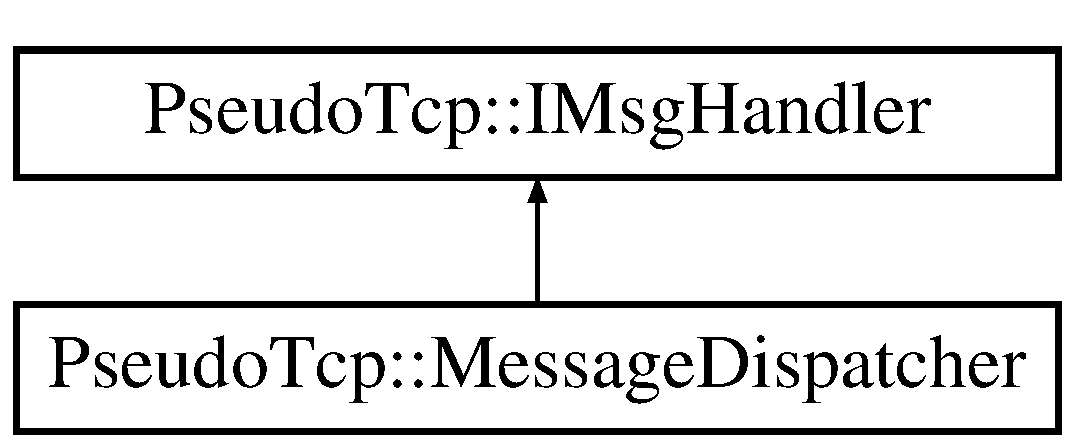
\includegraphics[height=2cm]{classPseudoTcp_1_1MessageDispatcher}
\end{center}
\end{figure}
\subsection*{Public Member Functions}
\begin{DoxyCompactItemize}
\item 
\hypertarget{classPseudoTcp_1_1MessageDispatcher_a91ef8930a0d28de5d284b1181ad42076}{
{\bfseries MessageDispatcher} (\hyperlink{classPseudoTcp_1_1IConnection}{IConnection} $\ast$conn, int windowSize)}
\label{classPseudoTcp_1_1MessageDispatcher_a91ef8930a0d28de5d284b1181ad42076}

\item 
\hypertarget{classPseudoTcp_1_1MessageDispatcher_a920a8bb42f0574728a7d672c1fa7cfe5}{
void \hyperlink{classPseudoTcp_1_1MessageDispatcher_a920a8bb42f0574728a7d672c1fa7cfe5}{IncomingMessage} (\hyperlink{classPseudoTcp_1_1Message}{Message} $\ast$msg)}
\label{classPseudoTcp_1_1MessageDispatcher_a920a8bb42f0574728a7d672c1fa7cfe5}

\begin{DoxyCompactList}\small\item\em \hyperlink{classPseudoTcp_1_1IMsgHandler}{IMsgHandler} interface3. \item\end{DoxyCompactList}\item 
\hypertarget{classPseudoTcp_1_1MessageDispatcher_a94b5e3d31894cc9151637e50daa7540d}{
int \hyperlink{classPseudoTcp_1_1MessageDispatcher_a94b5e3d31894cc9151637e50daa7540d}{send} (\hyperlink{classPseudoTcp_1_1Message}{Message} $\ast$msg)}
\label{classPseudoTcp_1_1MessageDispatcher_a94b5e3d31894cc9151637e50daa7540d}

\begin{DoxyCompactList}\small\item\em facade for Tx \item\end{DoxyCompactList}\item 
\hypertarget{classPseudoTcp_1_1MessageDispatcher_a637a302fe06f9abba2cb32f2f9fa7081}{
bool \hyperlink{classPseudoTcp_1_1MessageDispatcher_a637a302fe06f9abba2cb32f2f9fa7081}{allMessagesAcked} ()}
\label{classPseudoTcp_1_1MessageDispatcher_a637a302fe06f9abba2cb32f2f9fa7081}

\begin{DoxyCompactList}\small\item\em facade for Tx \item\end{DoxyCompactList}\item 
\hypertarget{classPseudoTcp_1_1MessageDispatcher_a08b707e4f9c0528b39f1c1eb5b9a61ba}{
\hyperlink{classPseudoTcp_1_1Message}{Message} $\ast$ {\bfseries getNextMessage} ()}
\label{classPseudoTcp_1_1MessageDispatcher_a08b707e4f9c0528b39f1c1eb5b9a61ba}

\item 
\hypertarget{classPseudoTcp_1_1MessageDispatcher_a4b2636001000dc4400b3767c69f17e38}{
void {\bfseries SetId} (int id)}
\label{classPseudoTcp_1_1MessageDispatcher_a4b2636001000dc4400b3767c69f17e38}

\item 
\hypertarget{classPseudoTcp_1_1MessageDispatcher_a9f10aed4d1487c935012a8c0cb954add}{
int {\bfseries GetId} () const }
\label{classPseudoTcp_1_1MessageDispatcher_a9f10aed4d1487c935012a8c0cb954add}

\end{DoxyCompactItemize}
\subsection*{Friends}
\begin{DoxyCompactItemize}
\item 
\hypertarget{classPseudoTcp_1_1MessageDispatcher_adbc53f711c49498562b7a674451cd0ab}{
std::ostream \& {\bfseries operator$<$$<$} (std::ostream \&o, \hyperlink{classPseudoTcp_1_1MessageDispatcher}{MessageDispatcher} const \&md)}
\label{classPseudoTcp_1_1MessageDispatcher_adbc53f711c49498562b7a674451cd0ab}

\end{DoxyCompactItemize}


\subsection{Detailed Description}
Top level \hyperlink{namespacePseudoTcp}{PseudoTcp} object, which contains TX and TX parts. Has two primary purposes:
\begin{DoxyEnumerate}
\item Act as encapsulator and facade for \hyperlink{classPseudoTcp_1_1PseudoTcpTx}{PseudoTcpTx} and \hyperlink{classPseudoTcp_1_1PseudoTcpRx}{PseudoTcpRx}
\item Handle incoming messages, sending them to RX (if payload) or TX (if ack info) as needed. 
\end{DoxyEnumerate}

The documentation for this class was generated from the following files:\begin{DoxyCompactItemize}
\item 
MessageDispatcher.hpp\item 
MessageDispatcher.cpp\end{DoxyCompactItemize}

\hypertarget{classutils_1_1MovingBuffer}{
\section{utils::MovingBuffer$<$ T $>$ Class Template Reference}
\label{classutils_1_1MovingBuffer}\index{utils::MovingBuffer@{utils::MovingBuffer}}
}


\hyperlink{classutils_1_1MovingBuffer}{MovingBuffer} is a data structure useful for PseudoTcpRx.  




{\ttfamily \#include $<$MovingBuffer.hpp$>$}

\subsection*{Public Member Functions}
\begin{DoxyCompactItemize}
\item 
\hypertarget{classutils_1_1MovingBuffer_aca199bfe148e820a848890ff0a519106}{
\hyperlink{classutils_1_1MovingBuffer_aca199bfe148e820a848890ff0a519106}{MovingBuffer} (int bufferSize)}
\label{classutils_1_1MovingBuffer_aca199bfe148e820a848890ff0a519106}

\begin{DoxyCompactList}\small\item\em Initialze with specified buffer size. \item\end{DoxyCompactList}\item 
T $\ast$ \hyperlink{classutils_1_1MovingBuffer_a7e65ffd8a9f4a5c428906e1da1931677}{get} (int index)
\item 
\hypertarget{classutils_1_1MovingBuffer_abe649be205205a783620c2d140b15114}{
void \hyperlink{classutils_1_1MovingBuffer_abe649be205205a783620c2d140b15114}{put} (T $\ast$newElement, int index)}
\label{classutils_1_1MovingBuffer_abe649be205205a783620c2d140b15114}

\begin{DoxyCompactList}\small\item\em Add a new element into the structure at the given absolute index. \item\end{DoxyCompactList}\item 
T $\ast$ \hyperlink{classutils_1_1MovingBuffer_afe0ca8bb2226b0039a265efe9952ac64}{pop} ()
\item 
\hypertarget{classutils_1_1MovingBuffer_a2388032df8ddb8b3a88692a81aaf7786}{
T $\ast$ \hyperlink{classutils_1_1MovingBuffer_a2388032df8ddb8b3a88692a81aaf7786}{popIfNotEmpty} ()}
\label{classutils_1_1MovingBuffer_a2388032df8ddb8b3a88692a81aaf7786}

\begin{DoxyCompactList}\small\item\em pop iff the first element is not NULL. \item\end{DoxyCompactList}\item 
\hypertarget{classutils_1_1MovingBuffer_a2fed5ea3406b8d3cbfc127a8df3aae7f}{
int \hyperlink{classutils_1_1MovingBuffer_a2fed5ea3406b8d3cbfc127a8df3aae7f}{getFirstIndex} () const }
\label{classutils_1_1MovingBuffer_a2fed5ea3406b8d3cbfc127a8df3aae7f}

\begin{DoxyCompactList}\small\item\em accessor for FirstIndex property \item\end{DoxyCompactList}\end{DoxyCompactItemize}
\subsection*{Static Public Attributes}
\begin{DoxyCompactItemize}
\item 
\hypertarget{classutils_1_1MovingBuffer_a9c9b030de547b19116873e00245d8759}{
static const int {\bfseries MovingBuffer\_\-IndexUnderflow} = -\/1}
\label{classutils_1_1MovingBuffer_a9c9b030de547b19116873e00245d8759}

\item 
\hypertarget{classutils_1_1MovingBuffer_aba4edd7c6f3e2ed445a6303f0869473d}{
static const int {\bfseries MovingBuffer\_\-IndexOverflow} = -\/2}
\label{classutils_1_1MovingBuffer_aba4edd7c6f3e2ed445a6303f0869473d}

\end{DoxyCompactItemize}
\subsection*{Friends}
\begin{DoxyCompactItemize}
\item 
\hypertarget{classutils_1_1MovingBuffer_a044b6dc71a4e89dd3f1d721ff77c6d62}{
std::ostream \& {\bfseries operator$<$$<$} (std::ostream \&o, \hyperlink{classutils_1_1MovingBuffer}{MovingBuffer} const \&mb)}
\label{classutils_1_1MovingBuffer_a044b6dc71a4e89dd3f1d721ff77c6d62}

\end{DoxyCompactItemize}


\subsection{Detailed Description}
\subsubsection*{template$<$class T$>$ class utils::MovingBuffer$<$ T $>$}

\hyperlink{classutils_1_1MovingBuffer}{MovingBuffer} is a data structure useful for PseudoTcpRx. A \hyperlink{classutils_1_1MovingBuffer}{MovingBuffer} is useful for keeping track of sequentially numbered items which may not arrive in order. The items are partitioned into three groups:
\begin{DoxyEnumerate}
\item 0-\/(n-\/1): First n contiguous items.
\item n ... n + bufferSize: Window in which out-\/of-\/sequence items may be added.
\item the rest (numbers above this can't be handled if they arrive, they exceed the buffer size.
\end{DoxyEnumerate}

Use by PseudoTcpRx: PseudoTcpRx utilizes a moving buffer to maintain the Message objects received. Given uncertainties in the underlying Connection, there may be gaps. This data structure is useful for keeping track of which Messages have arrived.

\begin{Desc}
\item[\hyperlink{todo__todo000002}{Todo}]: perhaps convert vector to deque. explain the implementation a bit. There are two parts to the structure. A buffer holds numbered items. An integer represents the first index of the buffer. This also implicitly tells us that the first (firstIndex -\/ 1) items have all arrived. The user will probably want to remove items as soon as the first gap is filled, that is why there is a popIfNotEmpty function. \end{Desc}


\subsection{Member Function Documentation}
\hypertarget{classutils_1_1MovingBuffer_a7e65ffd8a9f4a5c428906e1da1931677}{
\index{utils::MovingBuffer@{utils::MovingBuffer}!get@{get}}
\index{get@{get}!utils::MovingBuffer@{utils::MovingBuffer}}
\subsubsection[{get}]{\setlength{\rightskip}{0pt plus 5cm}template$<$class T $>$ T $\ast$ {\bf utils::MovingBuffer}$<$ T $>$::get (int {\em index})\hspace{0.3cm}{\ttfamily  \mbox{[}inline\mbox{]}}}}
\label{classutils_1_1MovingBuffer_a7e65ffd8a9f4a5c428906e1da1931677}
Retreive an element. The index should be 'absolute'. Can only have a return value for objects which are in the current buffer. \hypertarget{classutils_1_1MovingBuffer_afe0ca8bb2226b0039a265efe9952ac64}{
\index{utils::MovingBuffer@{utils::MovingBuffer}!pop@{pop}}
\index{pop@{pop}!utils::MovingBuffer@{utils::MovingBuffer}}
\subsubsection[{pop}]{\setlength{\rightskip}{0pt plus 5cm}template$<$class T $>$ T $\ast$ {\bf utils::MovingBuffer}$<$ T $>$::pop ()\hspace{0.3cm}{\ttfamily  \mbox{[}inline\mbox{]}}}}
\label{classutils_1_1MovingBuffer_afe0ca8bb2226b0039a265efe9952ac64}
Removes (and returns) the first element of the buffer, and 'shifts' the buffer window. 

The documentation for this class was generated from the following files:\begin{DoxyCompactItemize}
\item 
MovingBuffer.hpp\item 
MovingBuffer.cpp\end{DoxyCompactItemize}

\hypertarget{structp2p__callbacks}{
\section{p2p\_\-callbacks Struct Reference}
\label{structp2p__callbacks}\index{p2p\_\-callbacks@{p2p\_\-callbacks}}
}
\subsection*{Public Attributes}
\begin{DoxyCompactItemize}
\item 
\hypertarget{structp2p__callbacks_a36af71a9af29231e97b8bb06bf6b9403}{
void($\ast$ {\bfseries onNewConnection} )(struct \hyperlink{structP2pConnection}{P2pConnection} $\ast$conn)}
\label{structp2p__callbacks_a36af71a9af29231e97b8bb06bf6b9403}

\item 
\hypertarget{structp2p__callbacks_a71f50a9121e8a180623c6bd957b827f0}{
int($\ast$ {\bfseries onNewConnectionRequest} )(struct \hyperlink{structP2pConnection}{P2pConnection} $\ast$conn)}
\label{structp2p__callbacks_a71f50a9121e8a180623c6bd957b827f0}

\item 
\hypertarget{structp2p__callbacks_a54ee4b7b01e856d7f75537413fce6fb7}{
void($\ast$ {\bfseries onIncomingMessage} )(struct \hyperlink{structP2pConnection}{P2pConnection} $\ast$conn, char $\ast$msg, unsigned size)}
\label{structp2p__callbacks_a54ee4b7b01e856d7f75537413fce6fb7}

\item 
\hypertarget{structp2p__callbacks_a74ecf2c586bb5733fd6efc086e0073a9}{
void($\ast$ {\bfseries onNewUsers} )(char $\ast$rsUserString)}
\label{structp2p__callbacks_a74ecf2c586bb5733fd6efc086e0073a9}

\end{DoxyCompactItemize}


The documentation for this struct was generated from the following file:\begin{DoxyCompactItemize}
\item 
p2pConnApi.h\end{DoxyCompactItemize}

\hypertarget{structP2pConnection}{
\section{P2pConnection Struct Reference}
\label{structP2pConnection}\index{P2pConnection@{P2pConnection}}
}
\subsection*{Public Attributes}
\begin{DoxyCompactItemize}
\item 
\hypertarget{structP2pConnection_a8eecf9c7c3f62345634d3e74b023132f}{
enum P2pConnectionStatus {\bfseries status}}
\label{structP2pConnection_a8eecf9c7c3f62345634d3e74b023132f}

\item 
\hypertarget{structP2pConnection_a6b746b85e04fa05a18686d71766567b3}{
int {\bfseries id}}
\label{structP2pConnection_a6b746b85e04fa05a18686d71766567b3}

\item 
\hypertarget{structP2pConnection_a9770ff786603ce7fa98ae8926db68c2c}{
char {\bfseries otherUser} \mbox{[}MAX\_\-NAME\_\-LENGTH\mbox{]}}
\label{structP2pConnection_a9770ff786603ce7fa98ae8926db68c2c}

\item 
\hypertarget{structP2pConnection_acb10e9af725eca3591e2f7ff5bab4116}{
struct \hyperlink{structP2pConnectionOptions}{P2pConnectionOptions} $\ast$ {\bfseries opt}}
\label{structP2pConnection_acb10e9af725eca3591e2f7ff5bab4116}

\item 
\hypertarget{structP2pConnection_a5ebd408367ac9c8952201594532b9486}{
pj\_\-ice\_\-strans $\ast$ {\bfseries icest}}
\label{structP2pConnection_a5ebd408367ac9c8952201594532b9486}

\item 
\hypertarget{structP2pConnection_a5bfc67de65c4a87e1b5102f8d0dd9d34}{
pj\_\-ice\_\-strans\_\-cfg {\bfseries ice\_\-cfg}}
\label{structP2pConnection_a5bfc67de65c4a87e1b5102f8d0dd9d34}

\item 
\hypertarget{structP2pConnection_a0d4397b78e4420f3ff02a3f392a3a339}{
struct \hyperlink{structP2pRemoteInfo}{P2pRemoteInfo} {\bfseries remInfo}}
\label{structP2pConnection_a0d4397b78e4420f3ff02a3f392a3a339}

\item 
\hypertarget{structP2pConnection_a3e7a2ecb97838853b19ca983f4711546}{
char {\bfseries contactInfo} \mbox{[}ContactInfoLen\mbox{]}}
\label{structP2pConnection_a3e7a2ecb97838853b19ca983f4711546}

\item 
\hypertarget{structP2pConnection_aa0c0a1ff5550911d81d881309d86d535}{
char {\bfseries remoteInfoString} \mbox{[}ContactInfoLen\mbox{]}}
\label{structP2pConnection_aa0c0a1ff5550911d81d881309d86d535}

\end{DoxyCompactItemize}


The documentation for this struct was generated from the following file:\begin{DoxyCompactItemize}
\item 
p2pConnApi.h\end{DoxyCompactItemize}

\hypertarget{structP2pConnectionOptions}{
\section{P2pConnectionOptions Struct Reference}
\label{structP2pConnectionOptions}\index{P2pConnectionOptions@{P2pConnectionOptions}}
}
\subsection*{Public Attributes}
\begin{DoxyCompactItemize}
\item 
\hypertarget{structP2pConnectionOptions_aa3fdf3178b382fd24225c9856144a7ae}{
unsigned {\bfseries comp\_\-cnt}}
\label{structP2pConnectionOptions_aa3fdf3178b382fd24225c9856144a7ae}

\item 
\hypertarget{structP2pConnectionOptions_ab7608d18c5dc608abf58edc099b6911b}{
pj\_\-str\_\-t {\bfseries ns}}
\label{structP2pConnectionOptions_ab7608d18c5dc608abf58edc099b6911b}

\item 
\hypertarget{structP2pConnectionOptions_aebb8bf7a5b5c0bf690f91c9a83fc405a}{
int {\bfseries max\_\-host}}
\label{structP2pConnectionOptions_aebb8bf7a5b5c0bf690f91c9a83fc405a}

\item 
\hypertarget{structP2pConnectionOptions_a4495e7a652f55999cd84847a70ac07e4}{
pj\_\-bool\_\-t {\bfseries regular}}
\label{structP2pConnectionOptions_a4495e7a652f55999cd84847a70ac07e4}

\item 
\hypertarget{structP2pConnectionOptions_ab378112c8f59bba49ef2d54c083e6427}{
pj\_\-str\_\-t {\bfseries stun\_\-srv}}
\label{structP2pConnectionOptions_ab378112c8f59bba49ef2d54c083e6427}

\item 
\hypertarget{structP2pConnectionOptions_aa0a96958c4cd6738ec2180df5a57e280}{
pj\_\-str\_\-t {\bfseries turn\_\-srv}}
\label{structP2pConnectionOptions_aa0a96958c4cd6738ec2180df5a57e280}

\item 
\hypertarget{structP2pConnectionOptions_a7bd0d9239fc17f933877334465715bed}{
pj\_\-bool\_\-t {\bfseries turn\_\-tcp}}
\label{structP2pConnectionOptions_a7bd0d9239fc17f933877334465715bed}

\item 
\hypertarget{structP2pConnectionOptions_a3f82fdb3ce2b3185de56d043029f43c3}{
pj\_\-str\_\-t {\bfseries turn\_\-username}}
\label{structP2pConnectionOptions_a3f82fdb3ce2b3185de56d043029f43c3}

\item 
\hypertarget{structP2pConnectionOptions_a84fc563db0bbd3e4bc7222fe2f160636}{
pj\_\-str\_\-t {\bfseries turn\_\-password}}
\label{structP2pConnectionOptions_a84fc563db0bbd3e4bc7222fe2f160636}

\item 
\hypertarget{structP2pConnectionOptions_a995e2db2298d3b1286b18b9e87f8e6ef}{
pj\_\-bool\_\-t {\bfseries turn\_\-fingerprint}}
\label{structP2pConnectionOptions_a995e2db2298d3b1286b18b9e87f8e6ef}

\item 
\hypertarget{structP2pConnectionOptions_adfb6f71a25a33568517c016e47321180}{
const char $\ast$ {\bfseries log\_\-file}}
\label{structP2pConnectionOptions_adfb6f71a25a33568517c016e47321180}

\end{DoxyCompactItemize}


The documentation for this struct was generated from the following file:\begin{DoxyCompactItemize}
\item 
p2pConnApi.h\end{DoxyCompactItemize}

\hypertarget{structP2pRemoteInfo}{
\section{P2pRemoteInfo Struct Reference}
\label{structP2pRemoteInfo}\index{P2pRemoteInfo@{P2pRemoteInfo}}
}
\subsection*{Public Attributes}
\begin{DoxyCompactItemize}
\item 
\hypertarget{structP2pRemoteInfo_aeb023a14c460f4d5960e36a9dc10e06d}{
char {\bfseries ufrag} \mbox{[}80\mbox{]}}
\label{structP2pRemoteInfo_aeb023a14c460f4d5960e36a9dc10e06d}

\item 
\hypertarget{structP2pRemoteInfo_a24beff169e62368cca939e3904d0d914}{
char {\bfseries pwd} \mbox{[}80\mbox{]}}
\label{structP2pRemoteInfo_a24beff169e62368cca939e3904d0d914}

\item 
\hypertarget{structP2pRemoteInfo_a120bff9a641498f19b3f8728d4d1eb80}{
unsigned {\bfseries comp\_\-cnt}}
\label{structP2pRemoteInfo_a120bff9a641498f19b3f8728d4d1eb80}

\item 
\hypertarget{structP2pRemoteInfo_a8c750f28ffc2384ca473d318d02d484f}{
pj\_\-sockaddr {\bfseries def\_\-addr} \mbox{[}PJ\_\-ICE\_\-MAX\_\-COMP\mbox{]}}
\label{structP2pRemoteInfo_a8c750f28ffc2384ca473d318d02d484f}

\item 
\hypertarget{structP2pRemoteInfo_a9fe4fe3f796d2ed524332be099c0a2c8}{
unsigned {\bfseries cand\_\-cnt}}
\label{structP2pRemoteInfo_a9fe4fe3f796d2ed524332be099c0a2c8}

\item 
\hypertarget{structP2pRemoteInfo_a728680fe8a8b19af6605b9a6918d8393}{
pj\_\-ice\_\-sess\_\-cand {\bfseries cand} \mbox{[}PJ\_\-ICE\_\-ST\_\-MAX\_\-CAND\mbox{]}}
\label{structP2pRemoteInfo_a728680fe8a8b19af6605b9a6918d8393}

\end{DoxyCompactItemize}


The documentation for this struct was generated from the following file:\begin{DoxyCompactItemize}
\item 
p2pConnApi.h\end{DoxyCompactItemize}

\hypertarget{classPseudoTcp_1_1PseudoTcpRx}{
\section{PseudoTcp::PseudoTcpRx Class Reference}
\label{classPseudoTcp_1_1PseudoTcpRx}\index{PseudoTcp::PseudoTcpRx@{PseudoTcp::PseudoTcpRx}}
}


encapsulates RX part of protocol  




{\ttfamily \#include $<$PseudoTcpRx.hpp$>$}

Inheritance diagram for PseudoTcp::PseudoTcpRx:\begin{figure}[H]
\begin{center}
\leavevmode
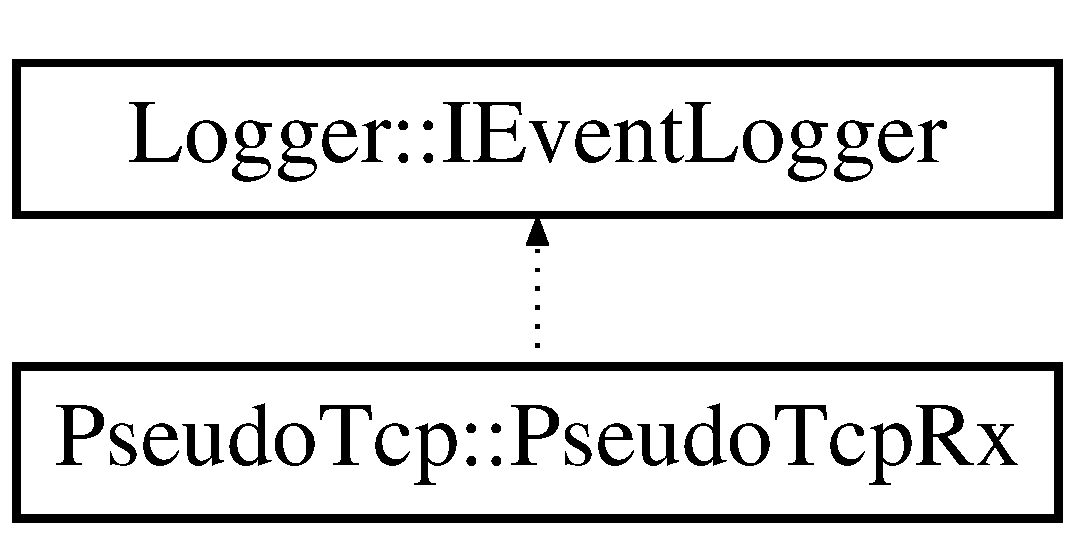
\includegraphics[height=2cm]{classPseudoTcp_1_1PseudoTcpRx}
\end{center}
\end{figure}
\subsection*{Public Member Functions}
\begin{DoxyCompactItemize}
\item 
\hypertarget{classPseudoTcp_1_1PseudoTcpRx_affb9c0ab2a36efac35367d2e3c79a489}{
{\bfseries PseudoTcpRx} (\hyperlink{classPseudoTcp_1_1PseudoTcpTx}{PseudoTcpTx} $\ast$tx, int msgBufferSize)}
\label{classPseudoTcp_1_1PseudoTcpRx_affb9c0ab2a36efac35367d2e3c79a489}

\item 
int \hyperlink{classPseudoTcp_1_1PseudoTcpRx_aa55a67cd15ae280201e8d0f0e669c7d1}{incomingMessage} (\hyperlink{classPseudoTcp_1_1Message}{Message} $\ast$msg)
\item 
void \hyperlink{classPseudoTcp_1_1PseudoTcpRx_a1aa8f7e24cb9f2874f1a64a09ee05a50}{sendAck} (\hyperlink{classPseudoTcp_1_1Message}{Message} $\ast$msg)
\item 
\hypertarget{classPseudoTcp_1_1PseudoTcpRx_a78415c5ad421240b7c703457895b6fdc}{
\hyperlink{classPseudoTcp_1_1Message}{Message} $\ast$ \hyperlink{classPseudoTcp_1_1PseudoTcpRx_a78415c5ad421240b7c703457895b6fdc}{getNextMessage} ()}
\label{classPseudoTcp_1_1PseudoTcpRx_a78415c5ad421240b7c703457895b6fdc}

\begin{DoxyCompactList}\small\item\em Returns next message in order. If none available, returns NULL;. \item\end{DoxyCompactList}\item 
\hypertarget{classPseudoTcp_1_1PseudoTcpRx_ab9917709e5c28986442be9723845ff41}{
\hyperlink{classPseudoTcp_1_1Message}{Message} $\ast$ {\bfseries getMessagesReceivedLog} ()}
\label{classPseudoTcp_1_1PseudoTcpRx_ab9917709e5c28986442be9723845ff41}

\item 
\hypertarget{classPseudoTcp_1_1PseudoTcpRx_a02a4c0427ffadb328662e04fdde80518}{
void {\bfseries setNextMsgIndex} (int nextMsgIndex)}
\label{classPseudoTcp_1_1PseudoTcpRx_a02a4c0427ffadb328662e04fdde80518}

\item 
\hypertarget{classPseudoTcp_1_1PseudoTcpRx_af42d85cc23fe516691cb38935b99945e}{
int {\bfseries getNextMsgIndex} () const }
\label{classPseudoTcp_1_1PseudoTcpRx_af42d85cc23fe516691cb38935b99945e}

\item 
\hypertarget{classPseudoTcp_1_1PseudoTcpRx_a9e1169de580b94339ad3bbcb7bd3559b}{
void {\bfseries setTestMode} (int testMode)}
\label{classPseudoTcp_1_1PseudoTcpRx_a9e1169de580b94339ad3bbcb7bd3559b}

\item 
\hypertarget{classPseudoTcp_1_1PseudoTcpRx_ae4ff932fdc6e913a59c7bb2f3cd14bd6}{
int {\bfseries getTestMode} () const }
\label{classPseudoTcp_1_1PseudoTcpRx_ae4ff932fdc6e913a59c7bb2f3cd14bd6}

\item 
\hypertarget{classPseudoTcp_1_1PseudoTcpRx_ada5eb147bc771df7dd4e32c11cc77c4c}{
void {\bfseries printState} (std::ostream \&o)}
\label{classPseudoTcp_1_1PseudoTcpRx_ada5eb147bc771df7dd4e32c11cc77c4c}

\item 
\hypertarget{classPseudoTcp_1_1PseudoTcpRx_abad5470549d03a14436775ac52acd7d0}{
std::string \hyperlink{classPseudoTcp_1_1PseudoTcpRx_abad5470549d03a14436775ac52acd7d0}{logString} ()}
\label{classPseudoTcp_1_1PseudoTcpRx_abad5470549d03a14436775ac52acd7d0}

\begin{DoxyCompactList}\small\item\em IEventLogger function. \item\end{DoxyCompactList}\item 
\hypertarget{classPseudoTcp_1_1PseudoTcpRx_aa85e034bcce1875d4295d96c54ab74a5}{
std::string \hyperlink{classPseudoTcp_1_1PseudoTcpRx_aa85e034bcce1875d4295d96c54ab74a5}{GetLogName} ()}
\label{classPseudoTcp_1_1PseudoTcpRx_aa85e034bcce1875d4295d96c54ab74a5}

\begin{DoxyCompactList}\small\item\em IEventLogger function. \item\end{DoxyCompactList}\item 
\hypertarget{classPseudoTcp_1_1PseudoTcpRx_a46d679252d77f1c7145fa03aae6597a2}{
void {\bfseries setId} (int id)}
\label{classPseudoTcp_1_1PseudoTcpRx_a46d679252d77f1c7145fa03aae6597a2}

\item 
\hypertarget{classPseudoTcp_1_1PseudoTcpRx_a0f1fc51ed563586383efd74afcd90bcf}{
int {\bfseries getId} () const }
\label{classPseudoTcp_1_1PseudoTcpRx_a0f1fc51ed563586383efd74afcd90bcf}

\end{DoxyCompactItemize}
\subsection*{Friends}
\begin{DoxyCompactItemize}
\item 
\hypertarget{classPseudoTcp_1_1PseudoTcpRx_af906343529e16495228f9852e1ca83c6}{
std::ostream \& {\bfseries operator$<$$<$} (std::ostream \&o, \hyperlink{classPseudoTcp_1_1PseudoTcpRx}{PseudoTcpRx} const \&rx)}
\label{classPseudoTcp_1_1PseudoTcpRx_af906343529e16495228f9852e1ca83c6}

\end{DoxyCompactItemize}


\subsection{Detailed Description}
encapsulates RX part of protocol The receiving end is responsable for:
\begin{DoxyEnumerate}
\item Ordering incoming messages
\item Making incoming messages available to higher level
\item Sending acks when needed 
\end{DoxyEnumerate}

\subsection{Member Function Documentation}
\hypertarget{classPseudoTcp_1_1PseudoTcpRx_aa55a67cd15ae280201e8d0f0e669c7d1}{
\index{PseudoTcp::PseudoTcpRx@{PseudoTcp::PseudoTcpRx}!incomingMessage@{incomingMessage}}
\index{incomingMessage@{incomingMessage}!PseudoTcp::PseudoTcpRx@{PseudoTcp::PseudoTcpRx}}
\subsubsection[{incomingMessage}]{\setlength{\rightskip}{0pt plus 5cm}int PseudoTcp::PseudoTcpRx::incomingMessage ({\bf Message} $\ast$ {\em msg})}}
\label{classPseudoTcp_1_1PseudoTcpRx_aa55a67cd15ae280201e8d0f0e669c7d1}
Callback for incoming message, called by \hyperlink{classPseudoTcp_1_1Connection}{Connection}. 
\begin{DoxyParams}{Parameters}
\item[{\em msg}]The message itself. \end{DoxyParams}
\begin{DoxyReturn}{Returns}
Number of bytes received. 
\end{DoxyReturn}
\hypertarget{classPseudoTcp_1_1PseudoTcpRx_a1aa8f7e24cb9f2874f1a64a09ee05a50}{
\index{PseudoTcp::PseudoTcpRx@{PseudoTcp::PseudoTcpRx}!sendAck@{sendAck}}
\index{sendAck@{sendAck}!PseudoTcp::PseudoTcpRx@{PseudoTcp::PseudoTcpRx}}
\subsubsection[{sendAck}]{\setlength{\rightskip}{0pt plus 5cm}void PseudoTcp::PseudoTcpRx::sendAck ({\bf Message} $\ast$ {\em msg})}}
\label{classPseudoTcp_1_1PseudoTcpRx_a1aa8f7e24cb9f2874f1a64a09ee05a50}
Send ack for \hyperlink{classPseudoTcp_1_1Message}{Message}. 
\begin{DoxyParams}{Parameters}
\item[{\em msg}]The \hyperlink{classPseudoTcp_1_1Message}{Message} to acknowledge. \end{DoxyParams}


The documentation for this class was generated from the following files:\begin{DoxyCompactItemize}
\item 
\hyperlink{PseudoTcpRx_8hpp}{PseudoTcpRx.hpp}\item 
PseudoTcpRx.cpp\end{DoxyCompactItemize}

\hypertarget{classPseudoTcp_1_1PseudoTcpTx}{
\section{PseudoTcp::PseudoTcpTx Class Reference}
\label{classPseudoTcp_1_1PseudoTcpTx}\index{PseudoTcp::PseudoTcpTx@{PseudoTcp::PseudoTcpTx}}
}


Encapsulates the sending half of the \hyperlink{namespacePseudoTcp}{PseudoTcp} protocol.  




{\ttfamily \#include $<$PseudoTcpTx.hpp$>$}

Inheritance diagram for PseudoTcp::PseudoTcpTx:\begin{figure}[H]
\begin{center}
\leavevmode
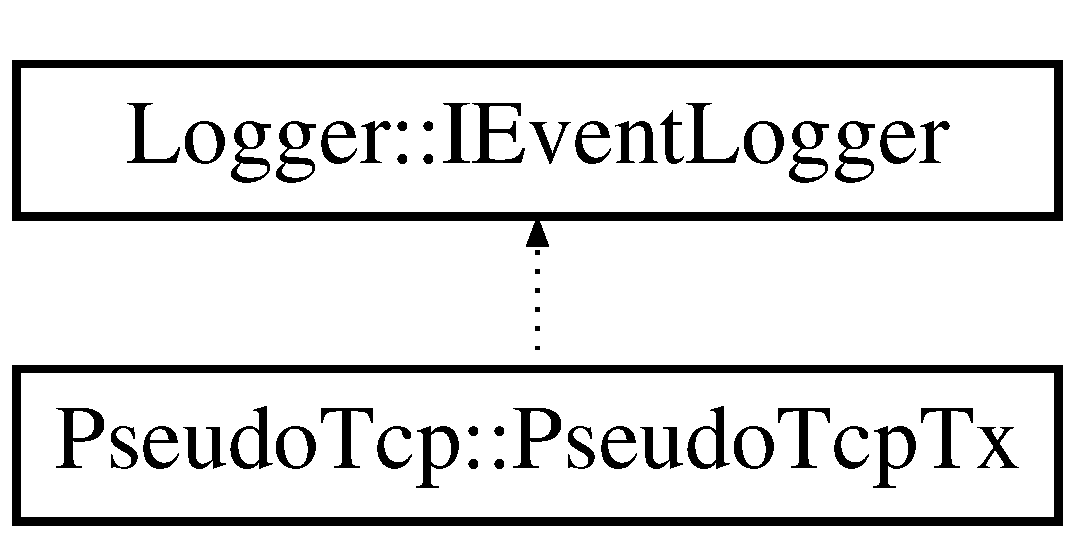
\includegraphics[height=2cm]{classPseudoTcp_1_1PseudoTcpTx}
\end{center}
\end{figure}
\subsection*{Public Member Functions}
\begin{DoxyCompactItemize}
\item 
\hypertarget{classPseudoTcp_1_1PseudoTcpTx_ac4a27695a1df46604d3b0b7b5e7a8626}{
{\bfseries PseudoTcpTx} (\hyperlink{classPseudoTcp_1_1IConnection}{IConnection} $\ast$conn, int msgBufferSize)}
\label{classPseudoTcp_1_1PseudoTcpTx_ac4a27695a1df46604d3b0b7b5e7a8626}

\item 
int \hyperlink{classPseudoTcp_1_1PseudoTcpTx_a647b783fb072921aa4451ee887644e34}{send} (\hyperlink{classPseudoTcp_1_1Message}{Message} $\ast$msg)
\item 
void \hyperlink{classPseudoTcp_1_1PseudoTcpTx_ab947a8457582a5647828bddaebca86a9}{incomingAck} (\hyperlink{classPseudoTcp_1_1Message}{Message} $\ast$msg)
\item 
\hypertarget{classPseudoTcp_1_1PseudoTcpTx_a9b3a72a495ab645207459d4cc6ebbdc2}{
int \hyperlink{classPseudoTcp_1_1PseudoTcpTx_a9b3a72a495ab645207459d4cc6ebbdc2}{getAcksReceived} () const }
\label{classPseudoTcp_1_1PseudoTcpTx_a9b3a72a495ab645207459d4cc6ebbdc2}

\begin{DoxyCompactList}\small\item\em this is just for debugging \item\end{DoxyCompactList}\item 
bool \hyperlink{classPseudoTcp_1_1PseudoTcpTx_a0285cf3faab1f34b97360bc9f4e68a77}{allMessagesAcked} ()
\item 
\hypertarget{classPseudoTcp_1_1PseudoTcpTx_a988c36108dc7eb80f8eeef220b78e5b8}{
void {\bfseries printState} (std::ostream \&o)}
\label{classPseudoTcp_1_1PseudoTcpTx_a988c36108dc7eb80f8eeef220b78e5b8}

\item 
\hypertarget{classPseudoTcp_1_1PseudoTcpTx_a3b36d6b9941b313755a9b099a6d0f077}{
void \hyperlink{classPseudoTcp_1_1PseudoTcpTx_a3b36d6b9941b313755a9b099a6d0f077}{startCheckAckThread} ()}
\label{classPseudoTcp_1_1PseudoTcpTx_a3b36d6b9941b313755a9b099a6d0f077}

\begin{DoxyCompactList}\small\item\em A thread which checks every ACK\_\-CHECKING\_\-INTERVAL msec for overdue acks. \item\end{DoxyCompactList}\item 
\hypertarget{classPseudoTcp_1_1PseudoTcpTx_a16e082eff985c8f985aa860dc2bc51e6}{
std::string {\bfseries logString} ()}
\label{classPseudoTcp_1_1PseudoTcpTx_a16e082eff985c8f985aa860dc2bc51e6}

\item 
\hypertarget{classPseudoTcp_1_1PseudoTcpTx_a6d3843b42bff2f5c2bf8e782bd6d2843}{
std::string {\bfseries GetLogName} ()}
\label{classPseudoTcp_1_1PseudoTcpTx_a6d3843b42bff2f5c2bf8e782bd6d2843}

\item 
\hypertarget{classPseudoTcp_1_1PseudoTcpTx_ae54c15a3b89ee9ef12370b3568863b8b}{
void {\bfseries setId} (int id)}
\label{classPseudoTcp_1_1PseudoTcpTx_ae54c15a3b89ee9ef12370b3568863b8b}

\item 
\hypertarget{classPseudoTcp_1_1PseudoTcpTx_a51eee9608065cbf4af43b764ea56bbcf}{
int {\bfseries getId} () const }
\label{classPseudoTcp_1_1PseudoTcpTx_a51eee9608065cbf4af43b764ea56bbcf}

\end{DoxyCompactItemize}
\subsection*{Friends}
\begin{DoxyCompactItemize}
\item 
\hypertarget{classPseudoTcp_1_1PseudoTcpTx_a70867e57670837e8e75b49c454fb2d60}{
std::ostream \& {\bfseries operator$<$$<$} (std::ostream \&o, \hyperlink{classPseudoTcp_1_1PseudoTcpTx}{PseudoTcpTx} const \&tx)}
\label{classPseudoTcp_1_1PseudoTcpTx_a70867e57670837e8e75b49c454fb2d60}

\end{DoxyCompactItemize}


\subsection{Detailed Description}
Encapsulates the sending half of the \hyperlink{namespacePseudoTcp}{PseudoTcp} protocol. The TX part is responsable for:
\begin{DoxyEnumerate}
\item Sending Messages, assigning \hyperlink{classPseudoTcp_1_1Message}{Message} number
\item Keeping track of which Messages have been acked
\item Keeping track of overdue acks
\item Resending Messages when necessary 
\end{DoxyEnumerate}

\subsection{Member Function Documentation}
\hypertarget{classPseudoTcp_1_1PseudoTcpTx_a0285cf3faab1f34b97360bc9f4e68a77}{
\index{PseudoTcp::PseudoTcpTx@{PseudoTcp::PseudoTcpTx}!allMessagesAcked@{allMessagesAcked}}
\index{allMessagesAcked@{allMessagesAcked}!PseudoTcp::PseudoTcpTx@{PseudoTcp::PseudoTcpTx}}
\subsubsection[{allMessagesAcked}]{\setlength{\rightskip}{0pt plus 5cm}bool PseudoTcp::PseudoTcpTx::allMessagesAcked ()\hspace{0.3cm}{\ttfamily  \mbox{[}inline\mbox{]}}}}
\label{classPseudoTcp_1_1PseudoTcpTx_a0285cf3faab1f34b97360bc9f4e68a77}
See if all messages have been send and acknowledged. \begin{DoxyReturn}{Returns}
true if they have. 
\end{DoxyReturn}
\hypertarget{classPseudoTcp_1_1PseudoTcpTx_ab947a8457582a5647828bddaebca86a9}{
\index{PseudoTcp::PseudoTcpTx@{PseudoTcp::PseudoTcpTx}!incomingAck@{incomingAck}}
\index{incomingAck@{incomingAck}!PseudoTcp::PseudoTcpTx@{PseudoTcp::PseudoTcpTx}}
\subsubsection[{incomingAck}]{\setlength{\rightskip}{0pt plus 5cm}void PseudoTcp::PseudoTcpTx::incomingAck ({\bf Message} $\ast$ {\em msg})}}
\label{classPseudoTcp_1_1PseudoTcpTx_ab947a8457582a5647828bddaebca86a9}
Update internal state based on information in ack, resending Messages and ack requests when necessary. 
\begin{DoxyParams}{Parameters}
\item[{\em msg}]\end{DoxyParams}
\hypertarget{classPseudoTcp_1_1PseudoTcpTx_a647b783fb072921aa4451ee887644e34}{
\index{PseudoTcp::PseudoTcpTx@{PseudoTcp::PseudoTcpTx}!send@{send}}
\index{send@{send}!PseudoTcp::PseudoTcpTx@{PseudoTcp::PseudoTcpTx}}
\subsubsection[{send}]{\setlength{\rightskip}{0pt plus 5cm}int PseudoTcp::PseudoTcpTx::send ({\bf Message} $\ast$ {\em msg})}}
\label{classPseudoTcp_1_1PseudoTcpTx_a647b783fb072921aa4451ee887644e34}
Send a message over the \hyperlink{classPseudoTcp_1_1Connection}{Connection}. 
\begin{DoxyParams}{Parameters}
\item[{\em msg}]The message to send. \end{DoxyParams}
\begin{DoxyReturn}{Returns}
1 if can be sent immediately, 2 if queued, -\/1 if buffer full, -\/2 if too big. 
\end{DoxyReturn}


The documentation for this class was generated from the following files:\begin{DoxyCompactItemize}
\item 
PseudoTcpTx.hpp\item 
PseudoTcpTx.cpp\end{DoxyCompactItemize}

\hypertarget{classSimpleTimer}{
\section{SimpleTimer Class Reference}
\label{classSimpleTimer}\index{SimpleTimer@{SimpleTimer}}
}
\subsection*{Public Member Functions}
\begin{DoxyCompactItemize}
\item 
\hypertarget{classSimpleTimer_ab46a9a774391760865df2d1c88d777cc}{
void {\bfseries restart} ()}
\label{classSimpleTimer_ab46a9a774391760865df2d1c88d777cc}

\item 
\hypertarget{classSimpleTimer_af4319404e506317898cce1d17b61be32}{
double {\bfseries elapsed} () const }
\label{classSimpleTimer_af4319404e506317898cce1d17b61be32}

\end{DoxyCompactItemize}
\subsection*{Static Public Member Functions}
\begin{DoxyCompactItemize}
\item 
\hypertarget{classSimpleTimer_a29a1e9d827950cb2471b15da06c0d1d1}{
static double {\bfseries now} ()}
\label{classSimpleTimer_a29a1e9d827950cb2471b15da06c0d1d1}

\end{DoxyCompactItemize}


The documentation for this class was generated from the following file:\begin{DoxyCompactItemize}
\item 
SimpleTimer.hpp\end{DoxyCompactItemize}

\chapter{File Documentation}
\hypertarget{mainpage_8h}{
\section{mainpage.h File Reference}
\label{mainpage_8h}\index{mainpage.h@{mainpage.h}}
}


Main page of Mymed peer-\/to-\/peer library documentation.  




\subsection{Detailed Description}
Main page of Mymed peer-\/to-\/peer library documentation. 
\hypertarget{PseudoTcpRx_8hpp}{
\section{PseudoTcpRx.hpp File Reference}
\label{PseudoTcpRx_8hpp}\index{PseudoTcpRx.hpp@{PseudoTcpRx.hpp}}
}
{\ttfamily \#include \char`\"{}MovingBuffer.hpp\char`\"{}}\par
{\ttfamily \#include \char`\"{}PseudoTcpUtil.hpp\char`\"{}}\par
{\ttfamily \#include \char`\"{}PseudoTcpTx.hpp\char`\"{}}\par
{\ttfamily \#include \char`\"{}EventLogger.hpp\char`\"{}}\par
{\ttfamily \#include $<$iostream$>$}\par
{\ttfamily \#include $<$sstream$>$}\par
{\ttfamily \#include $<$queue$>$}\par
\subsection*{Classes}
\begin{DoxyCompactItemize}
\item 
class \hyperlink{classPseudoTcp_1_1PseudoTcpRx}{PseudoTcp::PseudoTcpRx}
\begin{DoxyCompactList}\small\item\em encapsulates RX part of protocol \item\end{DoxyCompactList}\end{DoxyCompactItemize}
\subsection*{Namespaces}
\begin{DoxyCompactItemize}
\item 
namespace \hyperlink{namespacePseudoTcp}{PseudoTcp}


\begin{DoxyCompactList}\small\item\em The \hyperlink{namespacePseudoTcp}{PseudoTcp} namespace encapsulates the primary high-\/level objects involved in implementing the protocol. \item\end{DoxyCompactList}

\end{DoxyCompactItemize}
\subsection*{Defines}
\begin{DoxyCompactItemize}
\item 
\hypertarget{PseudoTcpRx_8hpp_a3ba2b8f2b16d288bb34f7fc32c4563f3}{
\#define {\bfseries MaxMessageLog}~1000}
\label{PseudoTcpRx_8hpp_a3ba2b8f2b16d288bb34f7fc32c4563f3}

\end{DoxyCompactItemize}


\subsection{Detailed Description}
PseudoTcpRx encapsulates the receiving half of the \hyperlink{namespacePseudoTcp}{PseudoTcp} protocol 
\printindex
\end{document}
